% Standalone compile harness for the ROS 2 chapter.
%
% This file approximates the CoreSense deliverable look (sans-serif body,
% teal accents, per-chapter float numbering) so the chapter can be built and
% reviewed independently. It is NOT part of the hand-over: the deliverable
% integrates ros2-chapter/ directly (see README.md).

\documentclass[11pt,a4paper]{report}

\usepackage[T1]{fontenc}
\usepackage[utf8]{inputenc}
\usepackage{lmodern}
\renewcommand{\familydefault}{\sfdefault}

\usepackage[a4paper,margin=2.6cm]{geometry}
\usepackage{microtype}
\usepackage{booktabs}
\usepackage{graphicx}
\usepackage{xcolor}
\usepackage{listings}
\usepackage{tikz}
\usetikzlibrary{positioning,arrows.meta,fit,backgrounds,calc}
\usepackage[ruled,linesnumbered,vlined]{algorithm2e}

% CoreSense-ish accent (teal like the D3.7 headings/links).
\definecolor{csTeal}{RGB}{0,106,113}
\usepackage[colorlinks=true,linkcolor=csTeal,urlcolor=csTeal,citecolor=csTeal]{hyperref}

% Chapter-specific additive definitions (colors, listing styles, tikz styles).
% The deliverable master must load this line in its preamble as well.
% Additive preamble for the ROS 2 chapter — load once in the master's preamble:
%   % Additive preamble for the ROS 2 chapter — load once in the master's preamble:
%   % Additive preamble for the ROS 2 chapter — load once in the master's preamble:
%   \input{ros2-chapter/chapter-preamble}
%
% Strictly additive and collision-safe: everything is ros2-prefixed, nothing
% global is redefined. Requires: xcolor, listings, tikz (positioning,
% arrows.meta, fit, backgrounds, calc), algorithm2e, booktabs.

\definecolor{ros2Accent}{RGB}{0,106,113}     % CoreSense teal
\definecolor{ros2Comment}{RGB}{90,110,120}   % muted slate for listing comments
\definecolor{ros2Frame}{RGB}{200,210,214}    % light rules around listings

% Style for ROS interface files (.msg/.srv/.action) and directory trees.
\lstdefinestyle{ros2iface}{
  basicstyle=\ttfamily\footnotesize,
  columns=fullflexible,
  keepspaces=true,
  showstringspaces=false,
  breaklines=true,
  breakatwhitespace=true,
  comment=[l]{\#},
  commentstyle=\color{ros2Comment}\itshape,
  frame=lines,
  rulecolor=\color{ros2Frame},
  aboveskip=0.8\baselineskip,
  belowskip=0.8\baselineskip,
}

% Style for shell sessions (build recipe, ros2 CLI walkthrough).
\lstdefinestyle{ros2shell}{
  language=bash,
  basicstyle=\ttfamily\footnotesize,
  columns=fullflexible,
  keepspaces=true,
  showstringspaces=false,
  breaklines=true,
  keywordstyle=\ttfamily\footnotesize,   % no keyword highlighting noise in shell
  comment=[l]{\#},
  commentstyle=\color{ros2Comment}\itshape,
  frame=lines,
  rulecolor=\color{ros2Frame},
  aboveskip=0.8\baselineskip,
  belowskip=0.8\baselineskip,
}

% Shared TikZ styles for the two chapter figures.
\tikzset{
  ros2/box/.style={draw, rounded corners=2pt, align=center, inner sep=5pt,
                   font=\footnotesize\sffamily},
  ros2/proc/.style={ros2/box, fill=ros2Accent!10, draw=ros2Accent},
  ros2/store/.style={ros2/box, fill=black!4, draw=black!45},
  ros2/state/.style={draw=ros2Accent, fill=ros2Accent!10, rounded corners=8pt,
                     align=center, inner sep=7pt, font=\footnotesize\sffamily\bfseries},
  ros2/arrow/.style={-{Stealth[length=2.4mm]}, thick, draw=black!70},
  ros2/accent arrow/.style={ros2/arrow, draw=ros2Accent},
  ros2/lbl/.style={font=\scriptsize\sffamily, align=center},
}

%
% Strictly additive and collision-safe: everything is ros2-prefixed, nothing
% global is redefined. Requires: xcolor, listings, tikz (positioning,
% arrows.meta, fit, backgrounds, calc), algorithm2e, booktabs.

\definecolor{ros2Accent}{RGB}{0,106,113}     % CoreSense teal
\definecolor{ros2Comment}{RGB}{90,110,120}   % muted slate for listing comments
\definecolor{ros2Frame}{RGB}{200,210,214}    % light rules around listings

% Style for ROS interface files (.msg/.srv/.action) and directory trees.
\lstdefinestyle{ros2iface}{
  basicstyle=\ttfamily\footnotesize,
  columns=fullflexible,
  keepspaces=true,
  showstringspaces=false,
  breaklines=true,
  breakatwhitespace=true,
  comment=[l]{\#},
  commentstyle=\color{ros2Comment}\itshape,
  frame=lines,
  rulecolor=\color{ros2Frame},
  aboveskip=0.8\baselineskip,
  belowskip=0.8\baselineskip,
}

% Style for shell sessions (build recipe, ros2 CLI walkthrough).
\lstdefinestyle{ros2shell}{
  language=bash,
  basicstyle=\ttfamily\footnotesize,
  columns=fullflexible,
  keepspaces=true,
  showstringspaces=false,
  breaklines=true,
  keywordstyle=\ttfamily\footnotesize,   % no keyword highlighting noise in shell
  comment=[l]{\#},
  commentstyle=\color{ros2Comment}\itshape,
  frame=lines,
  rulecolor=\color{ros2Frame},
  aboveskip=0.8\baselineskip,
  belowskip=0.8\baselineskip,
}

% Shared TikZ styles for the two chapter figures.
\tikzset{
  ros2/box/.style={draw, rounded corners=2pt, align=center, inner sep=5pt,
                   font=\footnotesize\sffamily},
  ros2/proc/.style={ros2/box, fill=ros2Accent!10, draw=ros2Accent},
  ros2/store/.style={ros2/box, fill=black!4, draw=black!45},
  ros2/state/.style={draw=ros2Accent, fill=ros2Accent!10, rounded corners=8pt,
                     align=center, inner sep=7pt, font=\footnotesize\sffamily\bfseries},
  ros2/arrow/.style={-{Stealth[length=2.4mm]}, thick, draw=black!70},
  ros2/accent arrow/.style={ros2/arrow, draw=ros2Accent},
  ros2/lbl/.style={font=\scriptsize\sffamily, align=center},
}

%
% Strictly additive and collision-safe: everything is ros2-prefixed, nothing
% global is redefined. Requires: xcolor, listings, tikz (positioning,
% arrows.meta, fit, backgrounds, calc), algorithm2e, booktabs.

\definecolor{ros2Accent}{RGB}{0,106,113}     % CoreSense teal
\definecolor{ros2Comment}{RGB}{90,110,120}   % muted slate for listing comments
\definecolor{ros2Frame}{RGB}{200,210,214}    % light rules around listings

% Style for ROS interface files (.msg/.srv/.action) and directory trees.
\lstdefinestyle{ros2iface}{
  basicstyle=\ttfamily\footnotesize,
  columns=fullflexible,
  keepspaces=true,
  showstringspaces=false,
  breaklines=true,
  breakatwhitespace=true,
  comment=[l]{\#},
  commentstyle=\color{ros2Comment}\itshape,
  frame=lines,
  rulecolor=\color{ros2Frame},
  aboveskip=0.8\baselineskip,
  belowskip=0.8\baselineskip,
}

% Style for shell sessions (build recipe, ros2 CLI walkthrough).
\lstdefinestyle{ros2shell}{
  language=bash,
  basicstyle=\ttfamily\footnotesize,
  columns=fullflexible,
  keepspaces=true,
  showstringspaces=false,
  breaklines=true,
  keywordstyle=\ttfamily\footnotesize,   % no keyword highlighting noise in shell
  comment=[l]{\#},
  commentstyle=\color{ros2Comment}\itshape,
  frame=lines,
  rulecolor=\color{ros2Frame},
  aboveskip=0.8\baselineskip,
  belowskip=0.8\baselineskip,
}

% Shared TikZ styles for the two chapter figures.
\tikzset{
  ros2/box/.style={draw, rounded corners=2pt, align=center, inner sep=5pt,
                   font=\footnotesize\sffamily},
  ros2/proc/.style={ros2/box, fill=ros2Accent!10, draw=ros2Accent},
  ros2/store/.style={ros2/box, fill=black!4, draw=black!45},
  ros2/state/.style={draw=ros2Accent, fill=ros2Accent!10, rounded corners=8pt,
                     align=center, inner sep=7pt, font=\footnotesize\sffamily\bfseries},
  ros2/arrow/.style={-{Stealth[length=2.4mm]}, thick, draw=black!70},
  ros2/accent arrow/.style={ros2/arrow, draw=ros2Accent},
  ros2/lbl/.style={font=\scriptsize\sffamily, align=center},
}


\begin{document}

% The ROS 2 chapter body. \input this from the deliverable master:
%   % The ROS 2 chapter body. \input this from the deliverable master:
%   % The ROS 2 chapter body. \input this from the deliverable master:
%   \input{ros2-chapter/chapter}
% Standard LaTeX only: no custom macros are defined or required beyond the
% additive styles in chapter-preamble.tex. All labels and citation keys are
% ros2:-prefixed to avoid collisions in the merged document.

\chapter{A ROS\,2 Module for Analytic Model Learning}
\label{ros2:chapter}

\section{Overview}
\label{ros2:sec:overview}

Deliverable D3.7~\cite{ros2:d37} introduced the Physics-Aware Modeling Module
(PhysicsAMM) and its symbolic-regression engine ANSR, and concluded with the
plan to expose the module as a ROS\,2 node following the best practices of the
CoreSense/ROS development guidelines D5.1~\cite{ros2:d51}. This chapter
documents that module. It consists of two ROS\,2 packages hosted in the
\texttt{ros2/} folder of the ANSR repository:

\begin{itemize}
  \item \texttt{physics\_amm} --- the wrapper node. It manages learning
        sessions, runs the unmodified ANSR core as a supervised subprocess,
        and serves the learned analytic models;
  \item \texttt{physics\_amm\_msgs} --- the interface definitions (messages,
        services, and one action), packaged separately as recommended by
        D5.1 for new interfaces.
\end{itemize}

D3.7 defined three operation modes for the module. Each maps onto exactly one
ROS\,2 interface:

\begin{itemize}
  \item \emph{Training a new model} --- the \texttt{learn\_model} action:
        a long-running, cancellable learning run with periodic feedback;
  \item \emph{Updating an existing model} --- the \texttt{set\_session\_data}
        service: the training data of a running session is replaced on the
        fly and the search adapts to the new data without a restart;
  \item \emph{Querying an existing model} --- the \texttt{get\_model}
        service: the current best-so-far analytic models are returned at any
        time, both during and after a learning run.
\end{itemize}

Learning and retrieval are deliberately decoupled: a learning run may take
minutes to hours, while a query returns immediately with the best models
found so far. The module targets ROS\,2 Jazzy Jalisco on Ubuntu~24.04
\cite{ros2:ros2science}, is released under the Apache-2.0 license, and ships
with a parameterised launcher, a configuration file of node parameters, and a
six-layer test suite (Section~\ref{ros2:sec:verification}).

\section{ANSR from an integration perspective}
\label{ros2:sec:core}

Four runtime characteristics of the ANSR core, described in the preceding
chapters and in~\cite{ros2:n4sr}, shape the design of the ROS layer:

\begin{enumerate}
  \item \textbf{Long-running, parallel computation.} A learning run is an
        asynchronous neuro-evolutionary search whose gradient-based
        coefficient tuning is distributed over a pool of worker processes
        (Dask~\cite{ros2:dask}, one PyTorch instance per worker). Runs last
        from minutes to hours, and the worker pool is managed dynamically
        over the course of a run.
  \item \textbf{File-based data interface.} Training and validation data are
        CSV files, and all inputs (data, master topology, optional
        constraints) are resolved relative to a structured working
        directory with dedicated subdirectories for each input kind.
  \item \textbf{Runtime data updates.} The core monitors its training-data
        file while the search is running. When the file changes, the data
        are reloaded, an internal \emph{dataset version} is advanced, and
        all fitness comparisons are made dataset-aware, so the search
        continues seamlessly on the new data.
  \item \textbf{Continuous best-so-far export.} The evolving populations are
        observable: the archive of non-dominated solutions and the live
        search population are continuously exported to disk, one snapshot
        directory per population and dataset version, refreshed whenever the
        populations improve (with a configurable minimum interval between
        refreshes).
\end{enumerate}

These characteristics are what make the three operation modes of
Section~\ref{ros2:sec:overview} natural to provide: the file-based interface
and runtime data monitoring directly support data exchange by file reference
and on-the-fly updates, and the continuous export makes best-so-far queries
possible without touching the running computation. The ROS layer builds on
each of them.

\section{Architecture}
\label{ros2:sec:architecture}

The module follows the session-based wrapper pattern established in the
CoreSense ecosystem by \texttt{coresense\_vampire}~\cite{ros2:vampire}, which
wraps another long-running computation (the Vampire theorem prover) behind a
session/action interface. Figure~\ref{ros2:fig:architecture} shows the
data flow.

\begin{figure}[tb]
  \centering
  \input{ros2-chapter/figures/fig-architecture}
  \caption{Architecture of the \texttt{physics\_amm} module. Clients interact
    with the node through four services and one action. Each learning session
    owns a private workspace; the ANSR core runs as a supervised subprocess
    with the workspace as its working directory and continuously exports its
    best-so-far models, which the node reads to serve queries and to publish
    action feedback.}
  \label{ros2:fig:architecture}
\end{figure}

\paragraph{Sessions.} All operations are scoped by a session: a client opens
a session (\texttt{start\_session}, returning a UUID), runs learning goals
and queries against it, and closes it (\texttt{end\_session}). Sessions
isolate concurrent users from each other: each session has its own workspace
and its own results directory.

\paragraph{Subprocess isolation.} The ANSR core runs in its own Python
process, launched and supervised by the node. This keeps the scientific
computing stack (PyTorch, Dask, SymPy) fully independent of the ROS
middleware process: the node itself performs no heavy computation in
callbacks --- in line with D5.1 --- and the core's worker pool is created in
a clean interpreter dedicated to the run. The subprocess is placed in its own
process group at launch, which lets the node manage the entire worker pool as
a single unit throughout the run (Section~\ref{ros2:sec:internals}).

\paragraph{Per-session workspaces.} For each learning goal, the node stages
the input files into a fresh workspace that reproduces the core's directory
conventions (\texttt{data/}, \texttt{topologies/}, \texttt{configs/},
\texttt{results/}) and starts the core with the workspace as its working
directory. Inputs are passed to the core by bare filename, exactly as in a
manual invocation. Staging copies the client's files, so later in-place data
updates never modify the originals.

\paragraph{Data by file reference.} Training data cross the ROS interface as
file paths rather than in-message payloads. This matches the core's
file-based data interface, keeps messages small, and makes the on-the-fly
data update (Section~\ref{ros2:sec:interfaces}) a natural operation: the node
replaces the staged file, and the core picks up the change through its
runtime data monitoring.

\paragraph{Minimal parameter surface.} Exactly five ANSR parameters are
exposed over ROS --- the master topology, the training and validation data,
an optional constraints file, and the results directory name. All remaining
settings use the defaults of the core's configuration, keeping the interface
deliberately small; node-level behaviour is configured separately through
ROS parameters (Section~\ref{ros2:sec:parameters}).

\paragraph{Guidelines compliance.} Following D5.1: the node package is plain
\texttt{ament\_python} with the recommended \texttt{setup.py} layout; new
interfaces live in the separate \texttt{physics\_amm\_msgs} package; the
node file is a thin ROS shim over ROS-agnostic, independently testable
modules (session staging, process supervision, result reading, session
registry); a parameterised Python launcher and a \texttt{config.yaml} of
default parameter values are provided; the license is Apache-2.0; and the
repository targets quality Tier~2 with a continuous-integration workflow.

\section{Interfaces}
\label{ros2:sec:interfaces}

Table~\ref{ros2:tab:interfaces} summarises the public interface of the node.
All names are relative to the node's namespace (\texttt{/physics\_amm} in the
default launch configuration).

\begin{table}[tb]
  \centering
  \caption{Public interface of the \texttt{physics\_amm} node. All types are
    defined in \texttt{physics\_amm\_msgs}.}
  \label{ros2:tab:interfaces}
  \footnotesize
  \begin{tabular}{@{}llll@{}}
    \toprule
    Name & Kind & Type & Purpose \\
    \midrule
    \texttt{start\_session}    & service & \texttt{StartSession}   & open a session; returns a UUID \\
    \texttt{end\_session}      & service & \texttt{EndSession}     & close a session, release its resources \\
    \texttt{learn\_model}      & action  & \texttt{LearnModel}     & run learning: long-running, cancellable \\
    \texttt{get\_model}        & service & \texttt{GetModel}       & query best-so-far analytic models \\
    \texttt{set\_session\_data}& service & \texttt{SetSessionData} & replace training data mid-run \\
    \bottomrule
  \end{tabular}
\end{table}

\subsection{The \texttt{LearnModel} action}
\label{ros2:sec:learnmodel}

Listing~\ref{ros2:lst:action} shows the complete action definition; the
in-file comments are part of the specification. The goal carries the session
id and the five ANSR parameters. Input paths are absolute paths on the host
running the node; the node stages them into the session workspace before the
run starts.

\begin{figure}[tb]
\lstinputlisting[style=ros2iface, caption={The \texttt{LearnModel} action
  definition (goal / result / feedback).},
  label={ros2:lst:action}]{ros2-chapter/listings/LearnModel.action}
\end{figure}

A goal is \emph{rejected} (not queued) if the session does not exist, an
input file is missing, or another learning run is currently active
(Section~\ref{ros2:sec:outlook}); rejection is immediate and retryable.
While the run executes, the node publishes feedback at a configurable period:
elapsed time, a status string, the current dataset version, and a summary of
the best model found so far (count, best validation loss, complexity).

The intended termination pattern is \emph{cancel when satisfied}: because
best-so-far models are available at any time through \texttt{get\_model},
a client typically monitors the feedback (or polls the query service) and
cancels the goal once the models are good enough. Cancellation is a
first-class action operation, is always accepted, and cleanly terminates the
whole computation (Section~\ref{ros2:sec:internals}). A run that is neither
cancelled nor stopped by the node-side wall-time watchdog ends when the
core's internal budget is exhausted; the result then carries
\texttt{CODE\_FINISHED} together with the final models.

\subsection{The \texttt{AnalyticModel} message}
\label{ros2:sec:analyticmodel}

Learned models are returned as \texttt{AnalyticModel} messages
(Table~\ref{ros2:tab:analyticmodel}), one per model. The message is
structurally parallel to \texttt{ModelDescription} in \texttt{coresense\_msgs},
so a later migration to the shared CoreSense types is a field mapping.

\begin{table}[tb]
  \centering
  \caption{Fields of \texttt{physics\_amm\_msgs/msg/AnalyticModel}.}
  \label{ros2:tab:analyticmodel}
  \footnotesize
  \begin{tabular}{@{}llp{7.2cm}@{}}
    \toprule
    Field & Type & Meaning \\
    \midrule
    \texttt{expression}            & \texttt{string}  & analytic formula in Python syntax \\
    \texttt{simplified\_expression}& \texttt{string}  & symbolically simplified form; may be empty \\
    \texttt{valid\_loss}           & \texttt{float64} & validation loss; NaN if not yet measured \\
    \texttt{complexity}            & \texttt{float64} & model complexity measure \\
    \texttt{num\_active\_nodes}    & \texttt{int32}   & active nodes in the topology; $-1$ if unknown \\
    \texttt{rmse\_constr}          & \texttt{float64} & constraint-compliance error; NaN if no constraints \\
    \texttt{dataset\_version}      & \texttt{uint32}  & dataset version of the snapshot the model comes from \\
    \texttt{population}            & \texttt{string}  & \texttt{archive} (non-dominated set) or \texttt{mainpop} \\
    \texttt{txt\_path}             & \texttt{string}  & path to the model's full text report \\
    \texttt{m\_path}               & \texttt{string}  & path to the MATLAB export of the formula \\
    \bottomrule
  \end{tabular}
\end{table}

\subsection{Session and retrieval services}
\label{ros2:sec:services}

The four services are intentionally small;
Table~\ref{ros2:tab:services} lists their request and response fields.

\begin{table}[tb]
  \centering
  \caption{Request and response fields of the session and retrieval services.
    All responses additionally carry \texttt{bool success} and
    \texttt{string message}.}
  \label{ros2:tab:services}
  \footnotesize
  \begin{tabular}{@{}lp{5.2cm}p{4.6cm}@{}}
    \toprule
    Service & Request & Response (besides status) \\
    \midrule
    \texttt{StartSession} & --- & \texttt{session\_id} (UUID) \\
    \addlinespace
    \texttt{EndSession} & \texttt{session\_id}; \texttt{force} & --- \\
    \addlinespace
    \texttt{GetModel} & \texttt{session\_id}; \texttt{population} (empty
      $=$ node default); \texttt{max\_models} ($0=$ all) &
      \texttt{dataset\_version}; \texttt{AnalyticModel[] models} \\
    \addlinespace
    \texttt{SetSessionData} & \texttt{session\_id};
      \texttt{train\_data\_path}; \texttt{valid\_data\_path} (empty $=$
      keep current) & --- \\
    \bottomrule
  \end{tabular}
\end{table}

\paragraph{Closing sessions.} \texttt{end\_session} with
\texttt{force:=false} refuses to close a session whose learning run is still
active --- a safeguard against accidentally destroying an ongoing
computation. With \texttt{force:=true}, the run is terminated first (through
the same clean mechanism as an action cancellation) and the session workspace
is then removed.

\paragraph{Querying models.} \texttt{get\_model} serves models from the
core's best-so-far export --- during a run, after it finishes, and after
cancellation. By default it reads the \emph{archive} (the non-dominated
solutions, i.e.\ the best accuracy--complexity trade-offs found so far); the
live search population is available by requesting
\texttt{population:=mainpop}. Because the export is refreshed at a minimum
interval (5\,s by default), a query may return a snapshot that is a few
seconds behind the live search state; this is documented behaviour and is
harmless for the best-so-far semantics of the call.

\paragraph{Updating data mid-run.} \texttt{set\_session\_data} implements the
\emph{updating an existing model} mode. The node copies the new file's
content over the staged training file --- atomically, preserving the staged
filename --- so the core's data monitoring observes the update, reloads the
data, and advances the dataset version. From that point on, models are
re-evaluated on the new data and the export continues under the new version.
The optional \texttt{valid\_data\_path} field updates the validation data in
the same way.

\section{Node parameters}
\label{ros2:sec:parameters}

Table~\ref{ros2:tab:params} lists all node parameters with their defaults
(from \texttt{config/params.yaml}, which also serves as the reference
configuration for the launcher).

\begin{table}[tb]
  \centering
  \caption{Parameters of the \texttt{physics\_amm} node.}
  \label{ros2:tab:params}
  \footnotesize
  \begin{tabular}{@{}llp{6.4cm}@{}}
    \toprule
    Parameter & Default & Meaning \\
    \midrule
    \texttt{workspace\_root} & \texttt{\textasciitilde/.ros/physics\_amm/sessions} &
      root directory for per-session workspaces \\
    \texttt{ansr\_source\_dir} & \emph{(installed copy)} &
      directory containing the ANSR core (\texttt{Main.py}) \\
    \texttt{python\_executable} & \emph{(node's interpreter)} &
      interpreter used for the ANSR subprocess \\
    \texttt{max\_concurrent\_runs} & \texttt{1} &
      learning runs executing at once (see Section~\ref{ros2:sec:outlook}) \\
    \texttt{max\_sessions} & \texttt{8} & open-session limit \\
    \texttt{sigterm\_grace\_s} & \texttt{10.0} &
      grace period in the two-stage run termination \\
    \texttt{feedback\_period\_s} & \texttt{2.0} &
      action feedback and cancellation-poll period \\
    \texttt{max\_run\_seconds} & \texttt{36000.0} &
      node-side wall-time watchdog ($0$ disables it) \\
    \texttt{default\_population} & \texttt{archive} &
      population served by \texttt{get\_model} when unspecified \\
    \texttt{mirror\_read\_retries} & \texttt{3} &
      re-reads of an export snapshot being refreshed \\
    \texttt{cleanup\_workspace\_on\_end} & \texttt{true} &
      remove the session workspace on \texttt{end\_session} \\
    \bottomrule
  \end{tabular}
\end{table}

Three parameters matter in practice. \texttt{python\_executable} selects the
interpreter for the ANSR subprocess and should point at the virtual
environment holding the scientific stack (Section~\ref{ros2:sec:usage});
\texttt{ansr\_source\_dir} overrides the packaged copy of the core with a
development checkout; and \texttt{workspace\_root} chooses where session
workspaces (staged data, logs, results) live --- by default under
\texttt{\textasciitilde/.ros}, the conventional location for node-private
state.

\section{Implementation internals}
\label{ros2:sec:internals}

The node file itself is a thin shim: all logic lives in four ROS-agnostic
modules --- \texttt{session} (workspace staging and command-line
construction), \texttt{supervisor} (subprocess lifecycle),
\texttt{results} (reading the best-so-far export), and
\texttt{session\_manager} (session registry and concurrency control) ---
which are unit-testable without a ROS installation. The node runs a
multi-threaded executor with two callback groups, so retrieval services
remain responsive while an action callback supervises a run.

\subsection{Session lifecycle}
\label{ros2:sec:lifecycle}

Figure~\ref{ros2:fig:lifecycle} shows the session state machine. A session is
\textsc{open} when created; it is \textsc{running} while a learning goal
executes and returns to \textsc{open} when the run ends --- its workspace and
results are retained, so \texttt{get\_model} continues to serve the learned
models. \texttt{end\_session} moves the session to the terminal
\textsc{ended} state and (by default) removes its workspace.

\begin{figure}[tb]
  \centering
  \input{ros2-chapter/figures/fig-lifecycle}
  \caption{Session lifecycle. A session returns to \textsc{open} after a run,
    keeping its results retrievable; closing it is an explicit, separate
    operation.}
  \label{ros2:fig:lifecycle}
\end{figure}

\subsection{Workspace staging and core invocation}
\label{ros2:sec:staging}

The workspace layout reproduces the core's directory conventions:

\begin{lstlisting}[style=ros2iface]
<session workspace>/
  data/         # training + validation CSV (staged copies)
  topologies/   # master topology file
  configs/      # constraints file (only when supplied)
  results/      # results directory targeted by the run
  logs/         # stdout/stderr of the ANSR subprocess
\end{lstlisting}

The core is invoked exactly as in a manual run: bare filenames for the
inputs, the workspace as the working directory, and only the five exposed
parameters on the command line. The subprocess environment pins the
numerical libraries to one thread per worker process
(\texttt{OMP\_NUM\_THREADS=1} and related variables), so the computational
footprint of a run equals its worker pool and remains predictable on a
shared robot computer. Staged copies also make the mid-run data update
self-contained: the update rewrites the staged file atomically under the
same name, which is precisely the event the core's data monitoring watches
for.

\subsection{Process supervision}
\label{ros2:sec:supervision}

A learning run is a small tree of processes: the core's main process, the
Dask scheduler it hosts, and the worker pool, whose members are recycled by
the core over the course of a run as part of its resource management. The
supervisor therefore manages the run at the granularity of its
\emph{process group}, which is invariant across worker recycling: the
subprocess is started as a new session leader, and all lifecycle operations
address the group as a whole.

Termination --- used by action cancellation, forced session closing, and the
wall-time watchdog alike --- follows the two-stage escalation of
Algorithm~\ref{ros2:alg:terminate}: a cooperative \texttt{SIGTERM} to the
whole group, a configurable grace period, then a definitive \texttt{SIGKILL}
for any remainder. The supervisor verifies that no process of the group
survives, so a cancelled run never leaves workers behind. This guarantee is
exercised by a dedicated integration test
(Section~\ref{ros2:sec:verification}).

\begin{algorithm}[tb]
  \caption{Two-stage termination of a learning run's process group.}
  \label{ros2:alg:terminate}
  \KwIn{process group $g$ of the run, grace period $T$}
  send \texttt{SIGTERM} to every process in $g$\;
  $t_{\mathrm{deadline}} \leftarrow \mathrm{now} + T$\;
  \While{$\mathrm{now} < t_{\mathrm{deadline}}$}{
    \lIf{no process of $g$ remains}{\Return}
    wait briefly\;
  }
  send \texttt{SIGKILL} to every process in $g$\;
  wait until no process of $g$ remains\;
\end{algorithm}

On the success path, the supervisor simply polls until the core exits and
tolerates the core's unhurried finalisation: the final export is already
complete on disk before the process ends, so the action result can be
assembled reliably. Exit classification distinguishes a completed run, a
cancelled run, and a failed run; in the failure case, the tail of the
subprocess log is attached to the action result's message for diagnosis. As
a safety net for unattended deployments, the node-side wall-time watchdog
(\texttt{max\_run\_seconds}) terminates a run through the same mechanism and
reports it as cancelled.

\subsection{Retrieving models from the export directory}
\label{ros2:sec:mirror}

Within a session's results directory, the core exports its best-so-far
models per population and dataset version:

\begin{lstlisting}[style=ros2iface]
<results>/seed=1/
  archiveIndividuals/current_best_<v>/          # non-dominated solutions
  mainPopulationIndividuals/current_best_<v>/   # live search population
\end{lstlisting}

Each snapshot directory holds one text report and one MATLAB export per
model, plus an overview file summarising the population. The reader
component selects the \emph{highest} version present --- after a mid-run
data update, a new version appears and earlier versions remain as snapshots
of the previous dataset --- and parses the overview together with the
per-model reports into \texttt{AnalyticModel} messages, preserving the
overview's ordering.

Two timing properties follow from the continuous-export design and are
handled by the reader. First, a snapshot that is being refreshed at the
moment of a query may be momentarily incomplete; reads are therefore retried
briefly and degrade gracefully to an empty result with an explanatory
message rather than failing. Second, the export interval bounds the
staleness of any answer (5\,s by default), and immediately after a data
update the new version's snapshot fills up as models are re-evaluated ---
clients polling right after \texttt{set\_session\_data} should expect the
new version to appear within a few export intervals.

\section{Building and running}
\label{ros2:sec:usage}

The module is built like any ROS\,2 workspace, with one addition: the ANSR
scientific stack (PyTorch, Dask, SymPy) lives in a Python virtual
environment created with system site-packages visible, so that both the ROS
client libraries and the scientific stack are importable from one
interpreter.

\begin{lstlisting}[style=ros2shell, caption={Build recipe (Ubuntu 24.04,
  ROS\,2 Jazzy).}, label={ros2:lst:build}]
sudo apt install ros-jazzy-ros-base python3.12-venv \
                 python3-colcon-common-extensions

# venv on the same interpreter ROS Jazzy uses (Python 3.12); the venv is
# used via absolute paths and never needs to be activated
python3.12 -m venv --system-site-packages ~/venvs/ansr

REPO=$(pwd)    # run from the repository root: absolute path for the steps below
~/venvs/ansr/bin/pip install -r $REPO/source_code/requirements.txt

source /opt/ros/jazzy/setup.bash

mkdir -p ~/ros2_ws/src
ln -sfn $REPO/ros2 ~/ros2_ws/src/physics_amm_ros
cd ~/ros2_ws && colcon build --symlink-install
source install/setup.bash    # repeat in every new terminal
\end{lstlisting}

The \texttt{python\_executable} launch argument (first line of
Listing~\ref{ros2:lst:cli}) points the ANSR subprocess at this virtual
environment's interpreter, so that the subprocess runs with the scientific
stack independently of which interpreter serves the node itself; the node
reports the effective interpreter in its startup log.
Listing~\ref{ros2:lst:cli} walks through a complete session with the
standard \texttt{ros2} command-line tools; the same calls are available
programmatically from any ROS\,2 client library.

\begin{lstlisting}[style=ros2shell, caption={A complete session from the
  command line.}, label={ros2:lst:cli}]
ros2 launch physics_amm physics_amm.launch.py \
     python_executable:=~/venvs/ansr/bin/python

# 1. open a session
ros2 service call /physics_amm/start_session \
     physics_amm_msgs/srv/StartSession

# 2. training a new model: send a learning goal (absolute paths)
ros2 action send_goal /physics_amm/learn_model \
     physics_amm_msgs/action/LearnModel \
     "{session_id: '<uuid>', topology_path: '<abs>/topology.txt',
       train_data_path: '<abs>/train.csv',
       valid_data_path: '<abs>/valid.csv',
       constraints_path: '', outfolder: results}" --feedback

# 3. querying: best-so-far models, any time during or after the run
ros2 service call /physics_amm/get_model \
     physics_amm_msgs/srv/GetModel \
     "{session_id: '<uuid>', population: '', max_models: 3}"

# 4. updating: replace the training data mid-run
ros2 service call /physics_amm/set_session_data \
     physics_amm_msgs/srv/SetSessionData \
     "{session_id: '<uuid>', train_data_path: '<abs>/new_train.csv',
       valid_data_path: ''}"

# 5. cancel when satisfied (Ctrl-C on send_goal, or the action API),
#    then close the session
ros2 service call /physics_amm/end_session \
     physics_amm_msgs/srv/EndSession \
     "{session_id: '<uuid>', force: true}"
\end{lstlisting}

Steps 2--4 are exactly the three operation modes announced in D3.7:
training, querying, and updating are one action goal and two service calls.
Data files are headerless comma-separated CSV with the target variable in
the last column.

\section{Verification}
\label{ros2:sec:verification}

ANSR is an asynchronous evolutionary method: the order in which tuned
candidates return from the worker pool depends on scheduling, so two runs
with identical inputs legitimately produce different (equally valid)
expressions. Verification of the ROS layer therefore does not compare
expressions or loss values against a reference run. Instead, the test suite
asserts the \emph{integration contract} --- that the node invokes and
observes the core exactly as a manual invocation would --- and
\emph{invariants} that must hold for any run. This is where integration
defects would actually appear: in the command line, the workspace layout,
the results path, or process lifecycle management, all of which are
deterministic and precisely testable.

Table~\ref{ros2:tab:tests} shows the six test layers.

The layers that execute the core share a set of bundled smoke fixtures:
60~training and 40~validation samples with inputs drawn uniformly from
$[-2,2]$ and \emph{noise-free} targets $y = x_0^2 + x_1$ (plus an alternative
dataset with $y = x_0^2 + 2x_1$ for the mid-run data update of layer~L5),
paired with a minimal master topology that can represent both targets
exactly. Short runs therefore converge to near-zero validation loss, which
keeps the ``did it learn anything?''\ assertions meaningful within
continuous-integration time budgets --- and any significant residual
implicates the integration, not the data.

\begin{table}[tb]
  \centering
  \caption{Test layers of the ROS bundle.}
  \label{ros2:tab:tests}
  \footnotesize
  \begin{tabular}{@{}clllp{5.1cm}@{}}
    \toprule
    \# & Layer & ROS & Speed & What it proves \\
    \midrule
    L1 & command-line contract & no  & ms         & the node invokes ANSR exactly as a human would \\
    L2 & workspace staging     & no  & ms         & the staged layout matches the core's conventions \\
    L3 & reference smoke       & no  & $\sim$1 min & baseline output structure of a direct run \\
    L4 & ROS smoke             & yes & $\sim$1 min & the action reproduces the L3 structure \\
    L5 & data update mid-run   & yes & $\sim$2 min & dataset version advances; queries answer mid-run \\
    L6 & cancellation          & yes & $\sim$30 s  & termination leaves no process of the run behind \\
    \bottomrule
  \end{tabular}
\end{table}

Layers L1 and L2 are fast, deterministic unit tests that run on every
commit; they pin the exact command line (only the five agreed parameters,
bare filenames) and the workspace layout. Layer L4 compares a run driven
through ROS against the direct-invocation baseline of L3 \emph{structurally}
--- same directory tree, same artifact kinds, finite losses --- never by
values. Layer L5 exercises the mid-run data update end-to-end and verifies
that queries are answered while the action is executing. Layer L6 verifies
the process-group termination guarantee of
Section~\ref{ros2:sec:supervision}: after a cancellation, no process of the
run's group remains within seconds. In addition, the packages carry unit
tests for the ROS-agnostic modules and a launch test that brings the node up
through its launcher, meeting the D5.1 requirement of testing both the
module API and the node; together the suites reach the coverage level of
quality Tier~2.

\section{Operational notes and outlook}
\label{ros2:sec:outlook}

\paragraph{One run at a time.} By default the node executes one learning run
at a time (parameter \texttt{max\_concurrent\_runs}, default~1); goals
arriving while a run is active are rejected immediately with an explanatory
message, and the client retries once the slot is free. Serialising runs keeps the CPU footprint of
the module equal to a single worker pool --- a deliberate choice for shared
robot computers, where the module coexists with perception and control. The
cap is a parameter, so a workstation deployment with ample cores may raise
it, giving each session its own isolated workspace and results directory.

\paragraph{Termination policy.} Learning is an anytime computation: the
best-so-far models are continuously available, so clients decide when the
result is good enough and cancel. The node-side watchdog
(\texttt{max\_run\_seconds}) bounds unattended runs; its default equals the
core's own time budget, so it acts purely as a safety net.

\paragraph{Outlook.} Three integration steps are foreseen. First, the
\texttt{AnalyticModel} message was designed field-compatible with
\texttt{ModelDescription} in \texttt{coresense\_msgs}, so migrating to the
shared CoreSense types once the consortium consolidates interfaces is a
mechanical mapping. Second, the module ships its own launcher and default
configuration, ready to be composed into a system-level bringup
(\texttt{coresense\_bringup}). Third, following the D5.1 release process,
the packages will be released with \texttt{bloom} from the
\texttt{jazzy-devel} branch once the interface has settled in consortium
use.

% Standard LaTeX only: no custom macros are defined or required beyond the
% additive styles in chapter-preamble.tex. All labels and citation keys are
% ros2:-prefixed to avoid collisions in the merged document.

\chapter{A ROS\,2 Module for Analytic Model Learning}
\label{ros2:chapter}

\section{Overview}
\label{ros2:sec:overview}

Deliverable D3.7~\cite{ros2:d37} introduced the Physics-Aware Modeling Module
(PhysicsAMM) and its symbolic-regression engine ANSR, and concluded with the
plan to expose the module as a ROS\,2 node following the best practices of the
CoreSense/ROS development guidelines D5.1~\cite{ros2:d51}. This chapter
documents that module. It consists of two ROS\,2 packages hosted in the
\texttt{ros2/} folder of the ANSR repository:

\begin{itemize}
  \item \texttt{physics\_amm} --- the wrapper node. It manages learning
        sessions, runs the unmodified ANSR core as a supervised subprocess,
        and serves the learned analytic models;
  \item \texttt{physics\_amm\_msgs} --- the interface definitions (messages,
        services, and one action), packaged separately as recommended by
        D5.1 for new interfaces.
\end{itemize}

D3.7 defined three operation modes for the module. Each maps onto exactly one
ROS\,2 interface:

\begin{itemize}
  \item \emph{Training a new model} --- the \texttt{learn\_model} action:
        a long-running, cancellable learning run with periodic feedback;
  \item \emph{Updating an existing model} --- the \texttt{set\_session\_data}
        service: the training data of a running session is replaced on the
        fly and the search adapts to the new data without a restart;
  \item \emph{Querying an existing model} --- the \texttt{get\_model}
        service: the current best-so-far analytic models are returned at any
        time, both during and after a learning run.
\end{itemize}

Learning and retrieval are deliberately decoupled: a learning run may take
minutes to hours, while a query returns immediately with the best models
found so far. The module targets ROS\,2 Jazzy Jalisco on Ubuntu~24.04
\cite{ros2:ros2science}, is released under the Apache-2.0 license, and ships
with a parameterised launcher, a configuration file of node parameters, and a
six-layer test suite (Section~\ref{ros2:sec:verification}).

\section{ANSR from an integration perspective}
\label{ros2:sec:core}

Four runtime characteristics of the ANSR core, described in the preceding
chapters and in~\cite{ros2:n4sr}, shape the design of the ROS layer:

\begin{enumerate}
  \item \textbf{Long-running, parallel computation.} A learning run is an
        asynchronous neuro-evolutionary search whose gradient-based
        coefficient tuning is distributed over a pool of worker processes
        (Dask~\cite{ros2:dask}, one PyTorch instance per worker). Runs last
        from minutes to hours, and the worker pool is managed dynamically
        over the course of a run.
  \item \textbf{File-based data interface.} Training and validation data are
        CSV files, and all inputs (data, master topology, optional
        constraints) are resolved relative to a structured working
        directory with dedicated subdirectories for each input kind.
  \item \textbf{Runtime data updates.} The core monitors its training-data
        file while the search is running. When the file changes, the data
        are reloaded, an internal \emph{dataset version} is advanced, and
        all fitness comparisons are made dataset-aware, so the search
        continues seamlessly on the new data.
  \item \textbf{Continuous best-so-far export.} The evolving populations are
        observable: the archive of non-dominated solutions and the live
        search population are continuously exported to disk, one snapshot
        directory per population and dataset version, refreshed whenever the
        populations improve (with a configurable minimum interval between
        refreshes).
\end{enumerate}

These characteristics are what make the three operation modes of
Section~\ref{ros2:sec:overview} natural to provide: the file-based interface
and runtime data monitoring directly support data exchange by file reference
and on-the-fly updates, and the continuous export makes best-so-far queries
possible without touching the running computation. The ROS layer builds on
each of them.

\section{Architecture}
\label{ros2:sec:architecture}

The module follows the session-based wrapper pattern established in the
CoreSense ecosystem by \texttt{coresense\_vampire}~\cite{ros2:vampire}, which
wraps another long-running computation (the Vampire theorem prover) behind a
session/action interface. Figure~\ref{ros2:fig:architecture} shows the
data flow.

\begin{figure}[tb]
  \centering
  % Architecture / data-flow figure. Bare tikzpicture; styles from chapter-preamble.
% Layout notes: every \\ line break sits at the TOP LEVEL of a node's text
% (TikZ's align machinery does not see breaks nested in brace groups), and all
% edge labels are anchored beside their line segments so no label crosses a
% line, a box border, or another label.
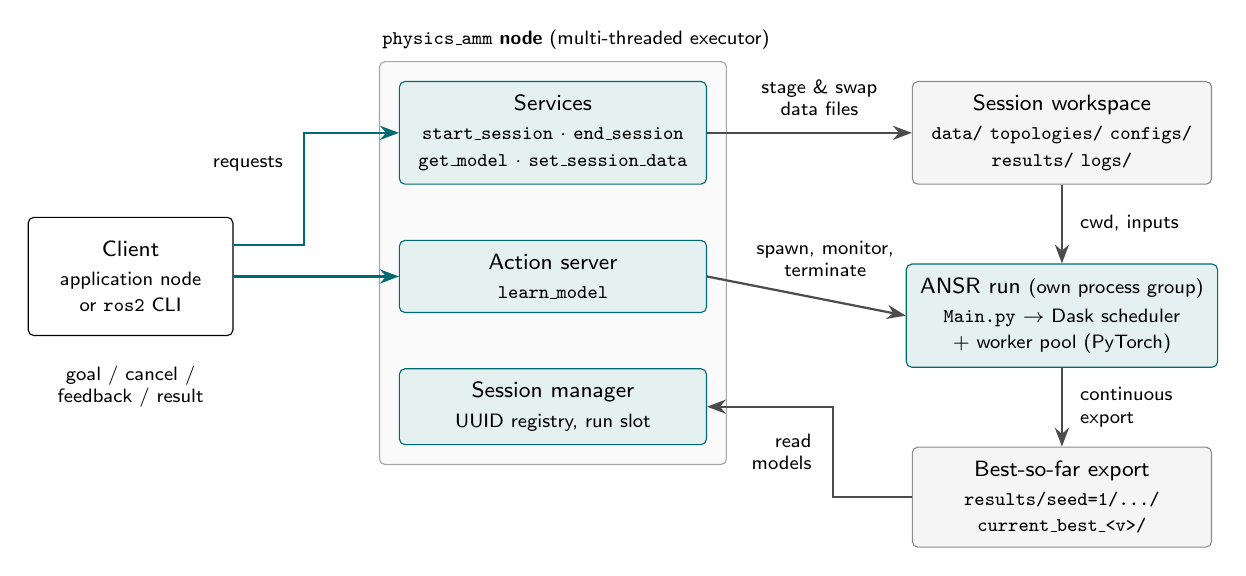
\begin{tikzpicture}

  % ---------------- node column ----------------
  \node[ros2/proc, minimum width=3.9cm] (services)
    {Services\\[1pt]
     {\scriptsize\texttt{start\_session} $\cdot$ \texttt{end\_session}}\\
     {\scriptsize\texttt{get\_model} $\cdot$ \texttt{set\_session\_data}}};
  \node[ros2/proc, below=7mm of services, minimum width=3.9cm] (action)
    {Action server\\[1pt]
     {\scriptsize\texttt{learn\_model}}};
  \node[ros2/proc, below=7mm of action, minimum width=3.9cm] (manager)
    {Session manager\\[1pt]
     {\scriptsize UUID registry, run slot}};

  \begin{scope}[on background layer]
    \node[ros2/box, fit=(services)(action)(manager), inner sep=7pt,
          fill=black!2, draw=black!35] (node) {};
  \end{scope}
  % Title anchored at the box's top-LEFT corner, away from the top-right
  % arrow label.
  \node[ros2/lbl, anchor=south west, inner sep=1pt]
    at ([yshift=1mm]node.north west)
    {\textbf{\texttt{physics\_amm} node} {\scriptsize(multi-threaded executor)}};

  % ---------------- client column ----------------
  \node[ros2/box, left=21mm of action, minimum width=2.6cm, minimum height=1.5cm]
    (client)
    {Client\\[1pt]
     {\scriptsize application node}\\
     {\scriptsize or \texttt{ros2} CLI}};

  % ---------------- session column ----------------
  \node[ros2/store, right=26mm of services, minimum width=3.8cm] (workspace)
    {Session workspace\\[1pt]
     {\scriptsize\texttt{data/}\ \texttt{topologies/}\ \texttt{configs/}}\\
     {\scriptsize\texttt{results/}\ \texttt{logs/}}};
  \node[ros2/proc, below=10mm of workspace, minimum width=3.8cm] (ansr)
    {ANSR run {\scriptsize(own process group)}\\[1pt]
     {\scriptsize\texttt{Main.py} $\rightarrow$ Dask scheduler}\\
     {\scriptsize$+$ worker pool (PyTorch)}};
  \node[ros2/store, below=10mm of ansr, minimum width=3.8cm] (mirror)
    {Best-so-far export\\[1pt]
     {\scriptsize\texttt{results/seed=1/\ldots/}}\\
     {\scriptsize\texttt{current\_best\_<v>/}}};

  % ---------------- client -> node edges ----------------
  % Elbow up to the services row; label sits left of the vertical riser,
  % well above the client box.
  \coordinate (reqcorner) at ([xshift=9mm, yshift=4mm]client.east);
  \coordinate (reqtop)    at (reqcorner |- services.west);
  \draw[ros2/accent arrow]
    ([yshift=4mm]client.east) -- (reqcorner) -- (reqtop) -- (services.west);
  \node[ros2/lbl, anchor=east, xshift=-1.5mm]
    at ($(reqcorner)!0.72!(reqtop)$) {requests};

  % Straight into the action row (client is centred on it); label below the
  % client box, clear of the arrow.
  \draw[ros2/accent arrow] (client.east) -- (action.west);
  \node[ros2/lbl, anchor=north, align=center]
    at ([yshift=-2.5mm]client.south)
    {goal / cancel /\\feedback / result};

  % ---------------- node <-> session edges ----------------
  \draw[ros2/arrow] (services.east) -- (workspace.west);
  \node[ros2/lbl, anchor=south, align=center, yshift=1mm]
    at ($(node.east |- services.east)!0.5!(workspace.west)$)
    {stage \& swap\\data files};

  \draw[ros2/arrow] (action.east) -- (ansr.west);
  \node[ros2/lbl, anchor=south, align=center, yshift=1.5mm]
    at ($(node.east |- action.east)!0.55!(ansr.west)$)
    {spawn, monitor,\\terminate};

  \coordinate (readcorner) at ([xshift=-10mm]mirror.west);
  \draw[ros2/arrow] (mirror.west) -- (readcorner) |- (manager.east);
  \node[ros2/lbl, anchor=east, align=right, xshift=-1.5mm]
    at ($(readcorner)!0.5!(readcorner |- manager.east)$)
    {read\\models};

  % ---------------- session column edges ----------------
  \draw[ros2/arrow] (workspace.south) -- (ansr.north)
    node[ros2/lbl, midway, right=1mm]{cwd, inputs};
  \draw[ros2/arrow] (ansr.south) -- (mirror.north)
    node[ros2/lbl, midway, right=1mm, align=left]{continuous\\export};

\end{tikzpicture}

  \caption{Architecture of the \texttt{physics\_amm} module. Clients interact
    with the node through four services and one action. Each learning session
    owns a private workspace; the ANSR core runs as a supervised subprocess
    with the workspace as its working directory and continuously exports its
    best-so-far models, which the node reads to serve queries and to publish
    action feedback.}
  \label{ros2:fig:architecture}
\end{figure}

\paragraph{Sessions.} All operations are scoped by a session: a client opens
a session (\texttt{start\_session}, returning a UUID), runs learning goals
and queries against it, and closes it (\texttt{end\_session}). Sessions
isolate concurrent users from each other: each session has its own workspace
and its own results directory.

\paragraph{Subprocess isolation.} The ANSR core runs in its own Python
process, launched and supervised by the node. This keeps the scientific
computing stack (PyTorch, Dask, SymPy) fully independent of the ROS
middleware process: the node itself performs no heavy computation in
callbacks --- in line with D5.1 --- and the core's worker pool is created in
a clean interpreter dedicated to the run. The subprocess is placed in its own
process group at launch, which lets the node manage the entire worker pool as
a single unit throughout the run (Section~\ref{ros2:sec:internals}).

\paragraph{Per-session workspaces.} For each learning goal, the node stages
the input files into a fresh workspace that reproduces the core's directory
conventions (\texttt{data/}, \texttt{topologies/}, \texttt{configs/},
\texttt{results/}) and starts the core with the workspace as its working
directory. Inputs are passed to the core by bare filename, exactly as in a
manual invocation. Staging copies the client's files, so later in-place data
updates never modify the originals.

\paragraph{Data by file reference.} Training data cross the ROS interface as
file paths rather than in-message payloads. This matches the core's
file-based data interface, keeps messages small, and makes the on-the-fly
data update (Section~\ref{ros2:sec:interfaces}) a natural operation: the node
replaces the staged file, and the core picks up the change through its
runtime data monitoring.

\paragraph{Minimal parameter surface.} Exactly five ANSR parameters are
exposed over ROS --- the master topology, the training and validation data,
an optional constraints file, and the results directory name. All remaining
settings use the defaults of the core's configuration, keeping the interface
deliberately small; node-level behaviour is configured separately through
ROS parameters (Section~\ref{ros2:sec:parameters}).

\paragraph{Guidelines compliance.} Following D5.1: the node package is plain
\texttt{ament\_python} with the recommended \texttt{setup.py} layout; new
interfaces live in the separate \texttt{physics\_amm\_msgs} package; the
node file is a thin ROS shim over ROS-agnostic, independently testable
modules (session staging, process supervision, result reading, session
registry); a parameterised Python launcher and a \texttt{config.yaml} of
default parameter values are provided; the license is Apache-2.0; and the
repository targets quality Tier~2 with a continuous-integration workflow.

\section{Interfaces}
\label{ros2:sec:interfaces}

Table~\ref{ros2:tab:interfaces} summarises the public interface of the node.
All names are relative to the node's namespace (\texttt{/physics\_amm} in the
default launch configuration).

\begin{table}[tb]
  \centering
  \caption{Public interface of the \texttt{physics\_amm} node. All types are
    defined in \texttt{physics\_amm\_msgs}.}
  \label{ros2:tab:interfaces}
  \footnotesize
  \begin{tabular}{@{}llll@{}}
    \toprule
    Name & Kind & Type & Purpose \\
    \midrule
    \texttt{start\_session}    & service & \texttt{StartSession}   & open a session; returns a UUID \\
    \texttt{end\_session}      & service & \texttt{EndSession}     & close a session, release its resources \\
    \texttt{learn\_model}      & action  & \texttt{LearnModel}     & run learning: long-running, cancellable \\
    \texttt{get\_model}        & service & \texttt{GetModel}       & query best-so-far analytic models \\
    \texttt{set\_session\_data}& service & \texttt{SetSessionData} & replace training data mid-run \\
    \bottomrule
  \end{tabular}
\end{table}

\subsection{The \texttt{LearnModel} action}
\label{ros2:sec:learnmodel}

Listing~\ref{ros2:lst:action} shows the complete action definition; the
in-file comments are part of the specification. The goal carries the session
id and the five ANSR parameters. Input paths are absolute paths on the host
running the node; the node stages them into the session workspace before the
run starts.

\begin{figure}[tb]
\lstinputlisting[style=ros2iface, caption={The \texttt{LearnModel} action
  definition (goal / result / feedback).},
  label={ros2:lst:action}]{ros2-chapter/listings/LearnModel.action}
\end{figure}

A goal is \emph{rejected} (not queued) if the session does not exist, an
input file is missing, or another learning run is currently active
(Section~\ref{ros2:sec:outlook}); rejection is immediate and retryable.
While the run executes, the node publishes feedback at a configurable period:
elapsed time, a status string, the current dataset version, and a summary of
the best model found so far (count, best validation loss, complexity).

The intended termination pattern is \emph{cancel when satisfied}: because
best-so-far models are available at any time through \texttt{get\_model},
a client typically monitors the feedback (or polls the query service) and
cancels the goal once the models are good enough. Cancellation is a
first-class action operation, is always accepted, and cleanly terminates the
whole computation (Section~\ref{ros2:sec:internals}). A run that is neither
cancelled nor stopped by the node-side wall-time watchdog ends when the
core's internal budget is exhausted; the result then carries
\texttt{CODE\_FINISHED} together with the final models.

\subsection{The \texttt{AnalyticModel} message}
\label{ros2:sec:analyticmodel}

Learned models are returned as \texttt{AnalyticModel} messages
(Table~\ref{ros2:tab:analyticmodel}), one per model. The message is
structurally parallel to \texttt{ModelDescription} in \texttt{coresense\_msgs},
so a later migration to the shared CoreSense types is a field mapping.

\begin{table}[tb]
  \centering
  \caption{Fields of \texttt{physics\_amm\_msgs/msg/AnalyticModel}.}
  \label{ros2:tab:analyticmodel}
  \footnotesize
  \begin{tabular}{@{}llp{7.2cm}@{}}
    \toprule
    Field & Type & Meaning \\
    \midrule
    \texttt{expression}            & \texttt{string}  & analytic formula in Python syntax \\
    \texttt{simplified\_expression}& \texttt{string}  & symbolically simplified form; may be empty \\
    \texttt{valid\_loss}           & \texttt{float64} & validation loss; NaN if not yet measured \\
    \texttt{complexity}            & \texttt{float64} & model complexity measure \\
    \texttt{num\_active\_nodes}    & \texttt{int32}   & active nodes in the topology; $-1$ if unknown \\
    \texttt{rmse\_constr}          & \texttt{float64} & constraint-compliance error; NaN if no constraints \\
    \texttt{dataset\_version}      & \texttt{uint32}  & dataset version of the snapshot the model comes from \\
    \texttt{population}            & \texttt{string}  & \texttt{archive} (non-dominated set) or \texttt{mainpop} \\
    \texttt{txt\_path}             & \texttt{string}  & path to the model's full text report \\
    \texttt{m\_path}               & \texttt{string}  & path to the MATLAB export of the formula \\
    \bottomrule
  \end{tabular}
\end{table}

\subsection{Session and retrieval services}
\label{ros2:sec:services}

The four services are intentionally small;
Table~\ref{ros2:tab:services} lists their request and response fields.

\begin{table}[tb]
  \centering
  \caption{Request and response fields of the session and retrieval services.
    All responses additionally carry \texttt{bool success} and
    \texttt{string message}.}
  \label{ros2:tab:services}
  \footnotesize
  \begin{tabular}{@{}lp{5.2cm}p{4.6cm}@{}}
    \toprule
    Service & Request & Response (besides status) \\
    \midrule
    \texttt{StartSession} & --- & \texttt{session\_id} (UUID) \\
    \addlinespace
    \texttt{EndSession} & \texttt{session\_id}; \texttt{force} & --- \\
    \addlinespace
    \texttt{GetModel} & \texttt{session\_id}; \texttt{population} (empty
      $=$ node default); \texttt{max\_models} ($0=$ all) &
      \texttt{dataset\_version}; \texttt{AnalyticModel[] models} \\
    \addlinespace
    \texttt{SetSessionData} & \texttt{session\_id};
      \texttt{train\_data\_path}; \texttt{valid\_data\_path} (empty $=$
      keep current) & --- \\
    \bottomrule
  \end{tabular}
\end{table}

\paragraph{Closing sessions.} \texttt{end\_session} with
\texttt{force:=false} refuses to close a session whose learning run is still
active --- a safeguard against accidentally destroying an ongoing
computation. With \texttt{force:=true}, the run is terminated first (through
the same clean mechanism as an action cancellation) and the session workspace
is then removed.

\paragraph{Querying models.} \texttt{get\_model} serves models from the
core's best-so-far export --- during a run, after it finishes, and after
cancellation. By default it reads the \emph{archive} (the non-dominated
solutions, i.e.\ the best accuracy--complexity trade-offs found so far); the
live search population is available by requesting
\texttt{population:=mainpop}. Because the export is refreshed at a minimum
interval (5\,s by default), a query may return a snapshot that is a few
seconds behind the live search state; this is documented behaviour and is
harmless for the best-so-far semantics of the call.

\paragraph{Updating data mid-run.} \texttt{set\_session\_data} implements the
\emph{updating an existing model} mode. The node copies the new file's
content over the staged training file --- atomically, preserving the staged
filename --- so the core's data monitoring observes the update, reloads the
data, and advances the dataset version. From that point on, models are
re-evaluated on the new data and the export continues under the new version.
The optional \texttt{valid\_data\_path} field updates the validation data in
the same way.

\section{Node parameters}
\label{ros2:sec:parameters}

Table~\ref{ros2:tab:params} lists all node parameters with their defaults
(from \texttt{config/params.yaml}, which also serves as the reference
configuration for the launcher).

\begin{table}[tb]
  \centering
  \caption{Parameters of the \texttt{physics\_amm} node.}
  \label{ros2:tab:params}
  \footnotesize
  \begin{tabular}{@{}llp{6.4cm}@{}}
    \toprule
    Parameter & Default & Meaning \\
    \midrule
    \texttt{workspace\_root} & \texttt{\textasciitilde/.ros/physics\_amm/sessions} &
      root directory for per-session workspaces \\
    \texttt{ansr\_source\_dir} & \emph{(installed copy)} &
      directory containing the ANSR core (\texttt{Main.py}) \\
    \texttt{python\_executable} & \emph{(node's interpreter)} &
      interpreter used for the ANSR subprocess \\
    \texttt{max\_concurrent\_runs} & \texttt{1} &
      learning runs executing at once (see Section~\ref{ros2:sec:outlook}) \\
    \texttt{max\_sessions} & \texttt{8} & open-session limit \\
    \texttt{sigterm\_grace\_s} & \texttt{10.0} &
      grace period in the two-stage run termination \\
    \texttt{feedback\_period\_s} & \texttt{2.0} &
      action feedback and cancellation-poll period \\
    \texttt{max\_run\_seconds} & \texttt{36000.0} &
      node-side wall-time watchdog ($0$ disables it) \\
    \texttt{default\_population} & \texttt{archive} &
      population served by \texttt{get\_model} when unspecified \\
    \texttt{mirror\_read\_retries} & \texttt{3} &
      re-reads of an export snapshot being refreshed \\
    \texttt{cleanup\_workspace\_on\_end} & \texttt{true} &
      remove the session workspace on \texttt{end\_session} \\
    \bottomrule
  \end{tabular}
\end{table}

Three parameters matter in practice. \texttt{python\_executable} selects the
interpreter for the ANSR subprocess and should point at the virtual
environment holding the scientific stack (Section~\ref{ros2:sec:usage});
\texttt{ansr\_source\_dir} overrides the packaged copy of the core with a
development checkout; and \texttt{workspace\_root} chooses where session
workspaces (staged data, logs, results) live --- by default under
\texttt{\textasciitilde/.ros}, the conventional location for node-private
state.

\section{Implementation internals}
\label{ros2:sec:internals}

The node file itself is a thin shim: all logic lives in four ROS-agnostic
modules --- \texttt{session} (workspace staging and command-line
construction), \texttt{supervisor} (subprocess lifecycle),
\texttt{results} (reading the best-so-far export), and
\texttt{session\_manager} (session registry and concurrency control) ---
which are unit-testable without a ROS installation. The node runs a
multi-threaded executor with two callback groups, so retrieval services
remain responsive while an action callback supervises a run.

\subsection{Session lifecycle}
\label{ros2:sec:lifecycle}

Figure~\ref{ros2:fig:lifecycle} shows the session state machine. A session is
\textsc{open} when created; it is \textsc{running} while a learning goal
executes and returns to \textsc{open} when the run ends --- its workspace and
results are retained, so \texttt{get\_model} continues to serve the learned
models. \texttt{end\_session} moves the session to the terminal
\textsc{ended} state and (by default) removes its workspace.

\begin{figure}[tb]
  \centering
  % Session lifecycle state machine. Bare tikzpicture; styles from chapter-preamble.
% Layout notes: \\ breaks at top level of node text only; transitions to ENDED
% are routed as elbows so their labels sit beside vertical segments, never on
% a line or a box.
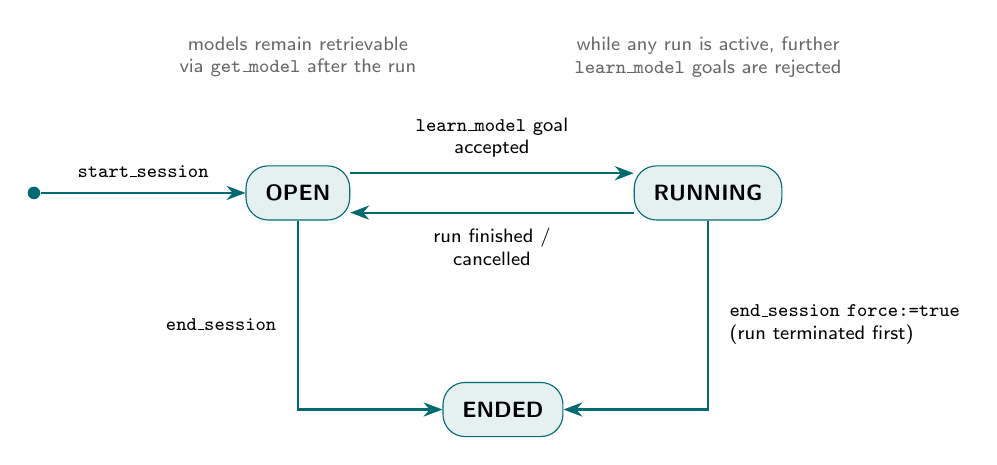
\begin{tikzpicture}

  \node[circle, fill=ros2Accent, inner sep=1.6pt] (init) {};
  \node[ros2/state, right=26mm of init] (open) {OPEN};
  \node[ros2/state, right=36mm of open] (running) {RUNNING};
  \node[ros2/state] (ended) at ($(open.south)!0.5!(running.south) + (0,-24mm)$) {ENDED};

  % ---------------- creation ----------------
  \draw[ros2/accent arrow] (init) -- (open)
    node[ros2/lbl, midway, above=0.7mm]{\texttt{start\_session}};

  % ---------------- OPEN <-> RUNNING ----------------
  \draw[ros2/accent arrow] ([yshift=2.5mm]open.east) -- ([yshift=2.5mm]running.west)
    node[ros2/lbl, midway, above=0.7mm, align=center]
    {\texttt{learn\_model} goal\\accepted};
  \draw[ros2/accent arrow] ([yshift=-2.5mm]running.west) -- ([yshift=-2.5mm]open.east)
    node[ros2/lbl, midway, below=0.7mm, align=center]{run finished /\\cancelled};

  % ---------------- closing ----------------
  % Elbows: straight down, then horizontally into ENDED; labels sit beside
  % the vertical segments.
  \coordinate (lcorner) at (open.south |- ended.west);
  \draw[ros2/accent arrow] (open.south) -- (lcorner) -- (ended.west);
  \node[ros2/lbl, anchor=east, xshift=-1.5mm]
    at ($(open.south)!0.55!(lcorner)$) {\texttt{end\_session}};

  \coordinate (rcorner) at (running.south |- ended.east);
  \draw[ros2/accent arrow] (running.south) -- (rcorner) -- (ended.east);
  \node[ros2/lbl, anchor=west, align=left, xshift=1.5mm]
    at ($(running.south)!0.55!(rcorner)$)
    {\texttt{end\_session} \texttt{force:=true}\\
     {\scriptsize(run terminated first)}};

  % ---------------- annotations ----------------
  \node[ros2/lbl, text=black!60, align=center, above=10mm of open.north]
    {models remain retrievable\\via \texttt{get\_model} after the run};
  \node[ros2/lbl, text=black!60, align=center, above=10mm of running.north]
    {while any run is active, further\\\texttt{learn\_model} goals are rejected};

\end{tikzpicture}

  \caption{Session lifecycle. A session returns to \textsc{open} after a run,
    keeping its results retrievable; closing it is an explicit, separate
    operation.}
  \label{ros2:fig:lifecycle}
\end{figure}

\subsection{Workspace staging and core invocation}
\label{ros2:sec:staging}

The workspace layout reproduces the core's directory conventions:

\begin{lstlisting}[style=ros2iface]
<session workspace>/
  data/         # training + validation CSV (staged copies)
  topologies/   # master topology file
  configs/      # constraints file (only when supplied)
  results/      # results directory targeted by the run
  logs/         # stdout/stderr of the ANSR subprocess
\end{lstlisting}

The core is invoked exactly as in a manual run: bare filenames for the
inputs, the workspace as the working directory, and only the five exposed
parameters on the command line. The subprocess environment pins the
numerical libraries to one thread per worker process
(\texttt{OMP\_NUM\_THREADS=1} and related variables), so the computational
footprint of a run equals its worker pool and remains predictable on a
shared robot computer. Staged copies also make the mid-run data update
self-contained: the update rewrites the staged file atomically under the
same name, which is precisely the event the core's data monitoring watches
for.

\subsection{Process supervision}
\label{ros2:sec:supervision}

A learning run is a small tree of processes: the core's main process, the
Dask scheduler it hosts, and the worker pool, whose members are recycled by
the core over the course of a run as part of its resource management. The
supervisor therefore manages the run at the granularity of its
\emph{process group}, which is invariant across worker recycling: the
subprocess is started as a new session leader, and all lifecycle operations
address the group as a whole.

Termination --- used by action cancellation, forced session closing, and the
wall-time watchdog alike --- follows the two-stage escalation of
Algorithm~\ref{ros2:alg:terminate}: a cooperative \texttt{SIGTERM} to the
whole group, a configurable grace period, then a definitive \texttt{SIGKILL}
for any remainder. The supervisor verifies that no process of the group
survives, so a cancelled run never leaves workers behind. This guarantee is
exercised by a dedicated integration test
(Section~\ref{ros2:sec:verification}).

\begin{algorithm}[tb]
  \caption{Two-stage termination of a learning run's process group.}
  \label{ros2:alg:terminate}
  \KwIn{process group $g$ of the run, grace period $T$}
  send \texttt{SIGTERM} to every process in $g$\;
  $t_{\mathrm{deadline}} \leftarrow \mathrm{now} + T$\;
  \While{$\mathrm{now} < t_{\mathrm{deadline}}$}{
    \lIf{no process of $g$ remains}{\Return}
    wait briefly\;
  }
  send \texttt{SIGKILL} to every process in $g$\;
  wait until no process of $g$ remains\;
\end{algorithm}

On the success path, the supervisor simply polls until the core exits and
tolerates the core's unhurried finalisation: the final export is already
complete on disk before the process ends, so the action result can be
assembled reliably. Exit classification distinguishes a completed run, a
cancelled run, and a failed run; in the failure case, the tail of the
subprocess log is attached to the action result's message for diagnosis. As
a safety net for unattended deployments, the node-side wall-time watchdog
(\texttt{max\_run\_seconds}) terminates a run through the same mechanism and
reports it as cancelled.

\subsection{Retrieving models from the export directory}
\label{ros2:sec:mirror}

Within a session's results directory, the core exports its best-so-far
models per population and dataset version:

\begin{lstlisting}[style=ros2iface]
<results>/seed=1/
  archiveIndividuals/current_best_<v>/          # non-dominated solutions
  mainPopulationIndividuals/current_best_<v>/   # live search population
\end{lstlisting}

Each snapshot directory holds one text report and one MATLAB export per
model, plus an overview file summarising the population. The reader
component selects the \emph{highest} version present --- after a mid-run
data update, a new version appears and earlier versions remain as snapshots
of the previous dataset --- and parses the overview together with the
per-model reports into \texttt{AnalyticModel} messages, preserving the
overview's ordering.

Two timing properties follow from the continuous-export design and are
handled by the reader. First, a snapshot that is being refreshed at the
moment of a query may be momentarily incomplete; reads are therefore retried
briefly and degrade gracefully to an empty result with an explanatory
message rather than failing. Second, the export interval bounds the
staleness of any answer (5\,s by default), and immediately after a data
update the new version's snapshot fills up as models are re-evaluated ---
clients polling right after \texttt{set\_session\_data} should expect the
new version to appear within a few export intervals.

\section{Building and running}
\label{ros2:sec:usage}

The module is built like any ROS\,2 workspace, with one addition: the ANSR
scientific stack (PyTorch, Dask, SymPy) lives in a Python virtual
environment created with system site-packages visible, so that both the ROS
client libraries and the scientific stack are importable from one
interpreter.

\begin{lstlisting}[style=ros2shell, caption={Build recipe (Ubuntu 24.04,
  ROS\,2 Jazzy).}, label={ros2:lst:build}]
sudo apt install ros-jazzy-ros-base python3.12-venv \
                 python3-colcon-common-extensions

# venv on the same interpreter ROS Jazzy uses (Python 3.12); the venv is
# used via absolute paths and never needs to be activated
python3.12 -m venv --system-site-packages ~/venvs/ansr

REPO=$(pwd)    # run from the repository root: absolute path for the steps below
~/venvs/ansr/bin/pip install -r $REPO/source_code/requirements.txt

source /opt/ros/jazzy/setup.bash

mkdir -p ~/ros2_ws/src
ln -sfn $REPO/ros2 ~/ros2_ws/src/physics_amm_ros
cd ~/ros2_ws && colcon build --symlink-install
source install/setup.bash    # repeat in every new terminal
\end{lstlisting}

The \texttt{python\_executable} launch argument (first line of
Listing~\ref{ros2:lst:cli}) points the ANSR subprocess at this virtual
environment's interpreter, so that the subprocess runs with the scientific
stack independently of which interpreter serves the node itself; the node
reports the effective interpreter in its startup log.
Listing~\ref{ros2:lst:cli} walks through a complete session with the
standard \texttt{ros2} command-line tools; the same calls are available
programmatically from any ROS\,2 client library.

\begin{lstlisting}[style=ros2shell, caption={A complete session from the
  command line.}, label={ros2:lst:cli}]
ros2 launch physics_amm physics_amm.launch.py \
     python_executable:=~/venvs/ansr/bin/python

# 1. open a session
ros2 service call /physics_amm/start_session \
     physics_amm_msgs/srv/StartSession

# 2. training a new model: send a learning goal (absolute paths)
ros2 action send_goal /physics_amm/learn_model \
     physics_amm_msgs/action/LearnModel \
     "{session_id: '<uuid>', topology_path: '<abs>/topology.txt',
       train_data_path: '<abs>/train.csv',
       valid_data_path: '<abs>/valid.csv',
       constraints_path: '', outfolder: results}" --feedback

# 3. querying: best-so-far models, any time during or after the run
ros2 service call /physics_amm/get_model \
     physics_amm_msgs/srv/GetModel \
     "{session_id: '<uuid>', population: '', max_models: 3}"

# 4. updating: replace the training data mid-run
ros2 service call /physics_amm/set_session_data \
     physics_amm_msgs/srv/SetSessionData \
     "{session_id: '<uuid>', train_data_path: '<abs>/new_train.csv',
       valid_data_path: ''}"

# 5. cancel when satisfied (Ctrl-C on send_goal, or the action API),
#    then close the session
ros2 service call /physics_amm/end_session \
     physics_amm_msgs/srv/EndSession \
     "{session_id: '<uuid>', force: true}"
\end{lstlisting}

Steps 2--4 are exactly the three operation modes announced in D3.7:
training, querying, and updating are one action goal and two service calls.
Data files are headerless comma-separated CSV with the target variable in
the last column.

\section{Verification}
\label{ros2:sec:verification}

ANSR is an asynchronous evolutionary method: the order in which tuned
candidates return from the worker pool depends on scheduling, so two runs
with identical inputs legitimately produce different (equally valid)
expressions. Verification of the ROS layer therefore does not compare
expressions or loss values against a reference run. Instead, the test suite
asserts the \emph{integration contract} --- that the node invokes and
observes the core exactly as a manual invocation would --- and
\emph{invariants} that must hold for any run. This is where integration
defects would actually appear: in the command line, the workspace layout,
the results path, or process lifecycle management, all of which are
deterministic and precisely testable.

Table~\ref{ros2:tab:tests} shows the six test layers.

The layers that execute the core share a set of bundled smoke fixtures:
60~training and 40~validation samples with inputs drawn uniformly from
$[-2,2]$ and \emph{noise-free} targets $y = x_0^2 + x_1$ (plus an alternative
dataset with $y = x_0^2 + 2x_1$ for the mid-run data update of layer~L5),
paired with a minimal master topology that can represent both targets
exactly. Short runs therefore converge to near-zero validation loss, which
keeps the ``did it learn anything?''\ assertions meaningful within
continuous-integration time budgets --- and any significant residual
implicates the integration, not the data.

\begin{table}[tb]
  \centering
  \caption{Test layers of the ROS bundle.}
  \label{ros2:tab:tests}
  \footnotesize
  \begin{tabular}{@{}clllp{5.1cm}@{}}
    \toprule
    \# & Layer & ROS & Speed & What it proves \\
    \midrule
    L1 & command-line contract & no  & ms         & the node invokes ANSR exactly as a human would \\
    L2 & workspace staging     & no  & ms         & the staged layout matches the core's conventions \\
    L3 & reference smoke       & no  & $\sim$1 min & baseline output structure of a direct run \\
    L4 & ROS smoke             & yes & $\sim$1 min & the action reproduces the L3 structure \\
    L5 & data update mid-run   & yes & $\sim$2 min & dataset version advances; queries answer mid-run \\
    L6 & cancellation          & yes & $\sim$30 s  & termination leaves no process of the run behind \\
    \bottomrule
  \end{tabular}
\end{table}

Layers L1 and L2 are fast, deterministic unit tests that run on every
commit; they pin the exact command line (only the five agreed parameters,
bare filenames) and the workspace layout. Layer L4 compares a run driven
through ROS against the direct-invocation baseline of L3 \emph{structurally}
--- same directory tree, same artifact kinds, finite losses --- never by
values. Layer L5 exercises the mid-run data update end-to-end and verifies
that queries are answered while the action is executing. Layer L6 verifies
the process-group termination guarantee of
Section~\ref{ros2:sec:supervision}: after a cancellation, no process of the
run's group remains within seconds. In addition, the packages carry unit
tests for the ROS-agnostic modules and a launch test that brings the node up
through its launcher, meeting the D5.1 requirement of testing both the
module API and the node; together the suites reach the coverage level of
quality Tier~2.

\section{Operational notes and outlook}
\label{ros2:sec:outlook}

\paragraph{One run at a time.} By default the node executes one learning run
at a time (parameter \texttt{max\_concurrent\_runs}, default~1); goals
arriving while a run is active are rejected immediately with an explanatory
message, and the client retries once the slot is free. Serialising runs keeps the CPU footprint of
the module equal to a single worker pool --- a deliberate choice for shared
robot computers, where the module coexists with perception and control. The
cap is a parameter, so a workstation deployment with ample cores may raise
it, giving each session its own isolated workspace and results directory.

\paragraph{Termination policy.} Learning is an anytime computation: the
best-so-far models are continuously available, so clients decide when the
result is good enough and cancel. The node-side watchdog
(\texttt{max\_run\_seconds}) bounds unattended runs; its default equals the
core's own time budget, so it acts purely as a safety net.

\paragraph{Outlook.} Three integration steps are foreseen. First, the
\texttt{AnalyticModel} message was designed field-compatible with
\texttt{ModelDescription} in \texttt{coresense\_msgs}, so migrating to the
shared CoreSense types once the consortium consolidates interfaces is a
mechanical mapping. Second, the module ships its own launcher and default
configuration, ready to be composed into a system-level bringup
(\texttt{coresense\_bringup}). Third, following the D5.1 release process,
the packages will be released with \texttt{bloom} from the
\texttt{jazzy-devel} branch once the interface has settled in consortium
use.

% Standard LaTeX only: no custom macros are defined or required beyond the
% additive styles in chapter-preamble.tex. All labels and citation keys are
% ros2:-prefixed to avoid collisions in the merged document.

\chapter{A ROS\,2 Module for Analytic Model Learning}
\label{ros2:chapter}

\section{Overview}
\label{ros2:sec:overview}

Deliverable D3.7~\cite{ros2:d37} introduced the Physics-Aware Modeling Module
(PhysicsAMM) and its symbolic-regression engine ANSR, and concluded with the
plan to expose the module as a ROS\,2 node following the best practices of the
CoreSense/ROS development guidelines D5.1~\cite{ros2:d51}. This chapter
documents that module. It consists of two ROS\,2 packages hosted in the
\texttt{ros2/} folder of the ANSR repository:

\begin{itemize}
  \item \texttt{physics\_amm} --- the wrapper node. It manages learning
        sessions, runs the unmodified ANSR core as a supervised subprocess,
        and serves the learned analytic models;
  \item \texttt{physics\_amm\_msgs} --- the interface definitions (messages,
        services, and one action), packaged separately as recommended by
        D5.1 for new interfaces.
\end{itemize}

D3.7 defined three operation modes for the module. Each maps onto exactly one
ROS\,2 interface:

\begin{itemize}
  \item \emph{Training a new model} --- the \texttt{learn\_model} action:
        a long-running, cancellable learning run with periodic feedback;
  \item \emph{Updating an existing model} --- the \texttt{set\_session\_data}
        service: the training data of a running session is replaced on the
        fly and the search adapts to the new data without a restart;
  \item \emph{Querying an existing model} --- the \texttt{get\_model}
        service: the current best-so-far analytic models are returned at any
        time, both during and after a learning run.
\end{itemize}

Learning and retrieval are deliberately decoupled: a learning run may take
minutes to hours, while a query returns immediately with the best models
found so far. The module targets ROS\,2 Jazzy Jalisco on Ubuntu~24.04
\cite{ros2:ros2science}, is released under the Apache-2.0 license, and ships
with a parameterised launcher, a configuration file of node parameters, and a
six-layer test suite (Section~\ref{ros2:sec:verification}).

\section{ANSR from an integration perspective}
\label{ros2:sec:core}

Four runtime characteristics of the ANSR core, described in the preceding
chapters and in~\cite{ros2:n4sr}, shape the design of the ROS layer:

\begin{enumerate}
  \item \textbf{Long-running, parallel computation.} A learning run is an
        asynchronous neuro-evolutionary search whose gradient-based
        coefficient tuning is distributed over a pool of worker processes
        (Dask~\cite{ros2:dask}, one PyTorch instance per worker). Runs last
        from minutes to hours, and the worker pool is managed dynamically
        over the course of a run.
  \item \textbf{File-based data interface.} Training and validation data are
        CSV files, and all inputs (data, master topology, optional
        constraints) are resolved relative to a structured working
        directory with dedicated subdirectories for each input kind.
  \item \textbf{Runtime data updates.} The core monitors its training-data
        file while the search is running. When the file changes, the data
        are reloaded, an internal \emph{dataset version} is advanced, and
        all fitness comparisons are made dataset-aware, so the search
        continues seamlessly on the new data.
  \item \textbf{Continuous best-so-far export.} The evolving populations are
        observable: the archive of non-dominated solutions and the live
        search population are continuously exported to disk, one snapshot
        directory per population and dataset version, refreshed whenever the
        populations improve (with a configurable minimum interval between
        refreshes).
\end{enumerate}

These characteristics are what make the three operation modes of
Section~\ref{ros2:sec:overview} natural to provide: the file-based interface
and runtime data monitoring directly support data exchange by file reference
and on-the-fly updates, and the continuous export makes best-so-far queries
possible without touching the running computation. The ROS layer builds on
each of them.

\section{Architecture}
\label{ros2:sec:architecture}

The module follows the session-based wrapper pattern established in the
CoreSense ecosystem by \texttt{coresense\_vampire}~\cite{ros2:vampire}, which
wraps another long-running computation (the Vampire theorem prover) behind a
session/action interface. Figure~\ref{ros2:fig:architecture} shows the
data flow.

\begin{figure}[tb]
  \centering
  % Architecture / data-flow figure. Bare tikzpicture; styles from chapter-preamble.
% Layout notes: every \\ line break sits at the TOP LEVEL of a node's text
% (TikZ's align machinery does not see breaks nested in brace groups), and all
% edge labels are anchored beside their line segments so no label crosses a
% line, a box border, or another label.
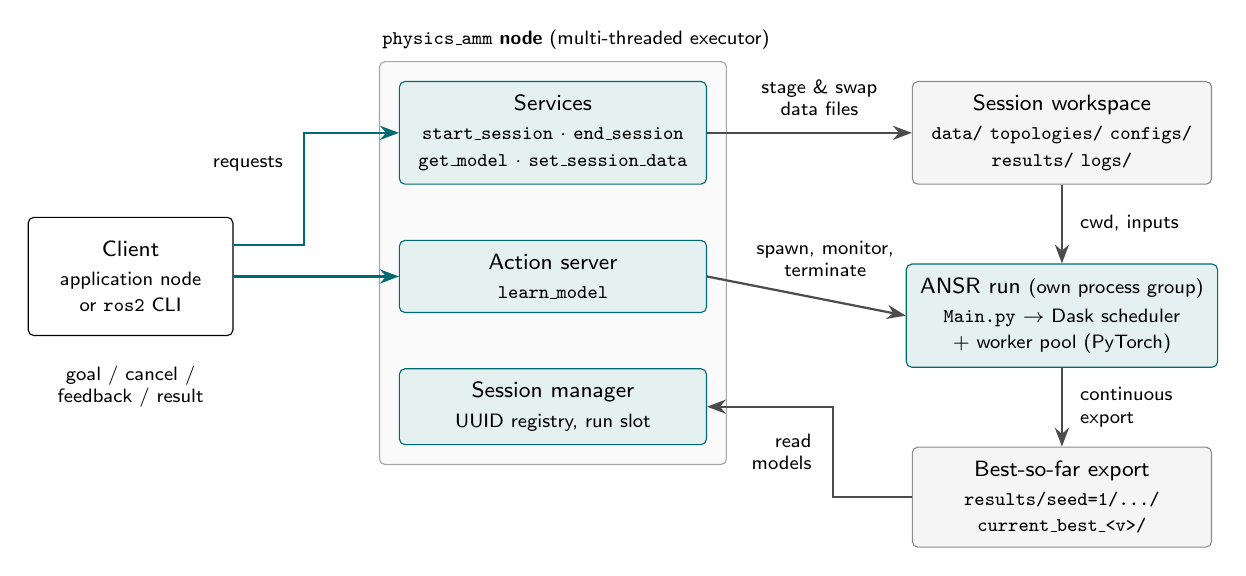
\begin{tikzpicture}

  % ---------------- node column ----------------
  \node[ros2/proc, minimum width=3.9cm] (services)
    {Services\\[1pt]
     {\scriptsize\texttt{start\_session} $\cdot$ \texttt{end\_session}}\\
     {\scriptsize\texttt{get\_model} $\cdot$ \texttt{set\_session\_data}}};
  \node[ros2/proc, below=7mm of services, minimum width=3.9cm] (action)
    {Action server\\[1pt]
     {\scriptsize\texttt{learn\_model}}};
  \node[ros2/proc, below=7mm of action, minimum width=3.9cm] (manager)
    {Session manager\\[1pt]
     {\scriptsize UUID registry, run slot}};

  \begin{scope}[on background layer]
    \node[ros2/box, fit=(services)(action)(manager), inner sep=7pt,
          fill=black!2, draw=black!35] (node) {};
  \end{scope}
  % Title anchored at the box's top-LEFT corner, away from the top-right
  % arrow label.
  \node[ros2/lbl, anchor=south west, inner sep=1pt]
    at ([yshift=1mm]node.north west)
    {\textbf{\texttt{physics\_amm} node} {\scriptsize(multi-threaded executor)}};

  % ---------------- client column ----------------
  \node[ros2/box, left=21mm of action, minimum width=2.6cm, minimum height=1.5cm]
    (client)
    {Client\\[1pt]
     {\scriptsize application node}\\
     {\scriptsize or \texttt{ros2} CLI}};

  % ---------------- session column ----------------
  \node[ros2/store, right=26mm of services, minimum width=3.8cm] (workspace)
    {Session workspace\\[1pt]
     {\scriptsize\texttt{data/}\ \texttt{topologies/}\ \texttt{configs/}}\\
     {\scriptsize\texttt{results/}\ \texttt{logs/}}};
  \node[ros2/proc, below=10mm of workspace, minimum width=3.8cm] (ansr)
    {ANSR run {\scriptsize(own process group)}\\[1pt]
     {\scriptsize\texttt{Main.py} $\rightarrow$ Dask scheduler}\\
     {\scriptsize$+$ worker pool (PyTorch)}};
  \node[ros2/store, below=10mm of ansr, minimum width=3.8cm] (mirror)
    {Best-so-far export\\[1pt]
     {\scriptsize\texttt{results/seed=1/\ldots/}}\\
     {\scriptsize\texttt{current\_best\_<v>/}}};

  % ---------------- client -> node edges ----------------
  % Elbow up to the services row; label sits left of the vertical riser,
  % well above the client box.
  \coordinate (reqcorner) at ([xshift=9mm, yshift=4mm]client.east);
  \coordinate (reqtop)    at (reqcorner |- services.west);
  \draw[ros2/accent arrow]
    ([yshift=4mm]client.east) -- (reqcorner) -- (reqtop) -- (services.west);
  \node[ros2/lbl, anchor=east, xshift=-1.5mm]
    at ($(reqcorner)!0.72!(reqtop)$) {requests};

  % Straight into the action row (client is centred on it); label below the
  % client box, clear of the arrow.
  \draw[ros2/accent arrow] (client.east) -- (action.west);
  \node[ros2/lbl, anchor=north, align=center]
    at ([yshift=-2.5mm]client.south)
    {goal / cancel /\\feedback / result};

  % ---------------- node <-> session edges ----------------
  \draw[ros2/arrow] (services.east) -- (workspace.west);
  \node[ros2/lbl, anchor=south, align=center, yshift=1mm]
    at ($(node.east |- services.east)!0.5!(workspace.west)$)
    {stage \& swap\\data files};

  \draw[ros2/arrow] (action.east) -- (ansr.west);
  \node[ros2/lbl, anchor=south, align=center, yshift=1.5mm]
    at ($(node.east |- action.east)!0.55!(ansr.west)$)
    {spawn, monitor,\\terminate};

  \coordinate (readcorner) at ([xshift=-10mm]mirror.west);
  \draw[ros2/arrow] (mirror.west) -- (readcorner) |- (manager.east);
  \node[ros2/lbl, anchor=east, align=right, xshift=-1.5mm]
    at ($(readcorner)!0.5!(readcorner |- manager.east)$)
    {read\\models};

  % ---------------- session column edges ----------------
  \draw[ros2/arrow] (workspace.south) -- (ansr.north)
    node[ros2/lbl, midway, right=1mm]{cwd, inputs};
  \draw[ros2/arrow] (ansr.south) -- (mirror.north)
    node[ros2/lbl, midway, right=1mm, align=left]{continuous\\export};

\end{tikzpicture}

  \caption{Architecture of the \texttt{physics\_amm} module. Clients interact
    with the node through four services and one action. Each learning session
    owns a private workspace; the ANSR core runs as a supervised subprocess
    with the workspace as its working directory and continuously exports its
    best-so-far models, which the node reads to serve queries and to publish
    action feedback.}
  \label{ros2:fig:architecture}
\end{figure}

\paragraph{Sessions.} All operations are scoped by a session: a client opens
a session (\texttt{start\_session}, returning a UUID), runs learning goals
and queries against it, and closes it (\texttt{end\_session}). Sessions
isolate concurrent users from each other: each session has its own workspace
and its own results directory.

\paragraph{Subprocess isolation.} The ANSR core runs in its own Python
process, launched and supervised by the node. This keeps the scientific
computing stack (PyTorch, Dask, SymPy) fully independent of the ROS
middleware process: the node itself performs no heavy computation in
callbacks --- in line with D5.1 --- and the core's worker pool is created in
a clean interpreter dedicated to the run. The subprocess is placed in its own
process group at launch, which lets the node manage the entire worker pool as
a single unit throughout the run (Section~\ref{ros2:sec:internals}).

\paragraph{Per-session workspaces.} For each learning goal, the node stages
the input files into a fresh workspace that reproduces the core's directory
conventions (\texttt{data/}, \texttt{topologies/}, \texttt{configs/},
\texttt{results/}) and starts the core with the workspace as its working
directory. Inputs are passed to the core by bare filename, exactly as in a
manual invocation. Staging copies the client's files, so later in-place data
updates never modify the originals.

\paragraph{Data by file reference.} Training data cross the ROS interface as
file paths rather than in-message payloads. This matches the core's
file-based data interface, keeps messages small, and makes the on-the-fly
data update (Section~\ref{ros2:sec:interfaces}) a natural operation: the node
replaces the staged file, and the core picks up the change through its
runtime data monitoring.

\paragraph{Minimal parameter surface.} Exactly five ANSR parameters are
exposed over ROS --- the master topology, the training and validation data,
an optional constraints file, and the results directory name. All remaining
settings use the defaults of the core's configuration, keeping the interface
deliberately small; node-level behaviour is configured separately through
ROS parameters (Section~\ref{ros2:sec:parameters}).

\paragraph{Guidelines compliance.} Following D5.1: the node package is plain
\texttt{ament\_python} with the recommended \texttt{setup.py} layout; new
interfaces live in the separate \texttt{physics\_amm\_msgs} package; the
node file is a thin ROS shim over ROS-agnostic, independently testable
modules (session staging, process supervision, result reading, session
registry); a parameterised Python launcher and a \texttt{config.yaml} of
default parameter values are provided; the license is Apache-2.0; and the
repository targets quality Tier~2 with a continuous-integration workflow.

\section{Interfaces}
\label{ros2:sec:interfaces}

Table~\ref{ros2:tab:interfaces} summarises the public interface of the node.
All names are relative to the node's namespace (\texttt{/physics\_amm} in the
default launch configuration).

\begin{table}[tb]
  \centering
  \caption{Public interface of the \texttt{physics\_amm} node. All types are
    defined in \texttt{physics\_amm\_msgs}.}
  \label{ros2:tab:interfaces}
  \footnotesize
  \begin{tabular}{@{}llll@{}}
    \toprule
    Name & Kind & Type & Purpose \\
    \midrule
    \texttt{start\_session}    & service & \texttt{StartSession}   & open a session; returns a UUID \\
    \texttt{end\_session}      & service & \texttt{EndSession}     & close a session, release its resources \\
    \texttt{learn\_model}      & action  & \texttt{LearnModel}     & run learning: long-running, cancellable \\
    \texttt{get\_model}        & service & \texttt{GetModel}       & query best-so-far analytic models \\
    \texttt{set\_session\_data}& service & \texttt{SetSessionData} & replace training data mid-run \\
    \bottomrule
  \end{tabular}
\end{table}

\subsection{The \texttt{LearnModel} action}
\label{ros2:sec:learnmodel}

Listing~\ref{ros2:lst:action} shows the complete action definition; the
in-file comments are part of the specification. The goal carries the session
id and the five ANSR parameters. Input paths are absolute paths on the host
running the node; the node stages them into the session workspace before the
run starts.

\begin{figure}[tb]
\lstinputlisting[style=ros2iface, caption={The \texttt{LearnModel} action
  definition (goal / result / feedback).},
  label={ros2:lst:action}]{ros2-chapter/listings/LearnModel.action}
\end{figure}

A goal is \emph{rejected} (not queued) if the session does not exist, an
input file is missing, or another learning run is currently active
(Section~\ref{ros2:sec:outlook}); rejection is immediate and retryable.
While the run executes, the node publishes feedback at a configurable period:
elapsed time, a status string, the current dataset version, and a summary of
the best model found so far (count, best validation loss, complexity).

The intended termination pattern is \emph{cancel when satisfied}: because
best-so-far models are available at any time through \texttt{get\_model},
a client typically monitors the feedback (or polls the query service) and
cancels the goal once the models are good enough. Cancellation is a
first-class action operation, is always accepted, and cleanly terminates the
whole computation (Section~\ref{ros2:sec:internals}). A run that is neither
cancelled nor stopped by the node-side wall-time watchdog ends when the
core's internal budget is exhausted; the result then carries
\texttt{CODE\_FINISHED} together with the final models.

\subsection{The \texttt{AnalyticModel} message}
\label{ros2:sec:analyticmodel}

Learned models are returned as \texttt{AnalyticModel} messages
(Table~\ref{ros2:tab:analyticmodel}), one per model. The message is
structurally parallel to \texttt{ModelDescription} in \texttt{coresense\_msgs},
so a later migration to the shared CoreSense types is a field mapping.

\begin{table}[tb]
  \centering
  \caption{Fields of \texttt{physics\_amm\_msgs/msg/AnalyticModel}.}
  \label{ros2:tab:analyticmodel}
  \footnotesize
  \begin{tabular}{@{}llp{7.2cm}@{}}
    \toprule
    Field & Type & Meaning \\
    \midrule
    \texttt{expression}            & \texttt{string}  & analytic formula in Python syntax \\
    \texttt{simplified\_expression}& \texttt{string}  & symbolically simplified form; may be empty \\
    \texttt{valid\_loss}           & \texttt{float64} & validation loss; NaN if not yet measured \\
    \texttt{complexity}            & \texttt{float64} & model complexity measure \\
    \texttt{num\_active\_nodes}    & \texttt{int32}   & active nodes in the topology; $-1$ if unknown \\
    \texttt{rmse\_constr}          & \texttt{float64} & constraint-compliance error; NaN if no constraints \\
    \texttt{dataset\_version}      & \texttt{uint32}  & dataset version of the snapshot the model comes from \\
    \texttt{population}            & \texttt{string}  & \texttt{archive} (non-dominated set) or \texttt{mainpop} \\
    \texttt{txt\_path}             & \texttt{string}  & path to the model's full text report \\
    \texttt{m\_path}               & \texttt{string}  & path to the MATLAB export of the formula \\
    \bottomrule
  \end{tabular}
\end{table}

\subsection{Session and retrieval services}
\label{ros2:sec:services}

The four services are intentionally small;
Table~\ref{ros2:tab:services} lists their request and response fields.

\begin{table}[tb]
  \centering
  \caption{Request and response fields of the session and retrieval services.
    All responses additionally carry \texttt{bool success} and
    \texttt{string message}.}
  \label{ros2:tab:services}
  \footnotesize
  \begin{tabular}{@{}lp{5.2cm}p{4.6cm}@{}}
    \toprule
    Service & Request & Response (besides status) \\
    \midrule
    \texttt{StartSession} & --- & \texttt{session\_id} (UUID) \\
    \addlinespace
    \texttt{EndSession} & \texttt{session\_id}; \texttt{force} & --- \\
    \addlinespace
    \texttt{GetModel} & \texttt{session\_id}; \texttt{population} (empty
      $=$ node default); \texttt{max\_models} ($0=$ all) &
      \texttt{dataset\_version}; \texttt{AnalyticModel[] models} \\
    \addlinespace
    \texttt{SetSessionData} & \texttt{session\_id};
      \texttt{train\_data\_path}; \texttt{valid\_data\_path} (empty $=$
      keep current) & --- \\
    \bottomrule
  \end{tabular}
\end{table}

\paragraph{Closing sessions.} \texttt{end\_session} with
\texttt{force:=false} refuses to close a session whose learning run is still
active --- a safeguard against accidentally destroying an ongoing
computation. With \texttt{force:=true}, the run is terminated first (through
the same clean mechanism as an action cancellation) and the session workspace
is then removed.

\paragraph{Querying models.} \texttt{get\_model} serves models from the
core's best-so-far export --- during a run, after it finishes, and after
cancellation. By default it reads the \emph{archive} (the non-dominated
solutions, i.e.\ the best accuracy--complexity trade-offs found so far); the
live search population is available by requesting
\texttt{population:=mainpop}. Because the export is refreshed at a minimum
interval (5\,s by default), a query may return a snapshot that is a few
seconds behind the live search state; this is documented behaviour and is
harmless for the best-so-far semantics of the call.

\paragraph{Updating data mid-run.} \texttt{set\_session\_data} implements the
\emph{updating an existing model} mode. The node copies the new file's
content over the staged training file --- atomically, preserving the staged
filename --- so the core's data monitoring observes the update, reloads the
data, and advances the dataset version. From that point on, models are
re-evaluated on the new data and the export continues under the new version.
The optional \texttt{valid\_data\_path} field updates the validation data in
the same way.

\section{Node parameters}
\label{ros2:sec:parameters}

Table~\ref{ros2:tab:params} lists all node parameters with their defaults
(from \texttt{config/params.yaml}, which also serves as the reference
configuration for the launcher).

\begin{table}[tb]
  \centering
  \caption{Parameters of the \texttt{physics\_amm} node.}
  \label{ros2:tab:params}
  \footnotesize
  \begin{tabular}{@{}llp{6.4cm}@{}}
    \toprule
    Parameter & Default & Meaning \\
    \midrule
    \texttt{workspace\_root} & \texttt{\textasciitilde/.ros/physics\_amm/sessions} &
      root directory for per-session workspaces \\
    \texttt{ansr\_source\_dir} & \emph{(installed copy)} &
      directory containing the ANSR core (\texttt{Main.py}) \\
    \texttt{python\_executable} & \emph{(node's interpreter)} &
      interpreter used for the ANSR subprocess \\
    \texttt{max\_concurrent\_runs} & \texttt{1} &
      learning runs executing at once (see Section~\ref{ros2:sec:outlook}) \\
    \texttt{max\_sessions} & \texttt{8} & open-session limit \\
    \texttt{sigterm\_grace\_s} & \texttt{10.0} &
      grace period in the two-stage run termination \\
    \texttt{feedback\_period\_s} & \texttt{2.0} &
      action feedback and cancellation-poll period \\
    \texttt{max\_run\_seconds} & \texttt{36000.0} &
      node-side wall-time watchdog ($0$ disables it) \\
    \texttt{default\_population} & \texttt{archive} &
      population served by \texttt{get\_model} when unspecified \\
    \texttt{mirror\_read\_retries} & \texttt{3} &
      re-reads of an export snapshot being refreshed \\
    \texttt{cleanup\_workspace\_on\_end} & \texttt{true} &
      remove the session workspace on \texttt{end\_session} \\
    \bottomrule
  \end{tabular}
\end{table}

Three parameters matter in practice. \texttt{python\_executable} selects the
interpreter for the ANSR subprocess and should point at the virtual
environment holding the scientific stack (Section~\ref{ros2:sec:usage});
\texttt{ansr\_source\_dir} overrides the packaged copy of the core with a
development checkout; and \texttt{workspace\_root} chooses where session
workspaces (staged data, logs, results) live --- by default under
\texttt{\textasciitilde/.ros}, the conventional location for node-private
state.

\section{Implementation internals}
\label{ros2:sec:internals}

The node file itself is a thin shim: all logic lives in four ROS-agnostic
modules --- \texttt{session} (workspace staging and command-line
construction), \texttt{supervisor} (subprocess lifecycle),
\texttt{results} (reading the best-so-far export), and
\texttt{session\_manager} (session registry and concurrency control) ---
which are unit-testable without a ROS installation. The node runs a
multi-threaded executor with two callback groups, so retrieval services
remain responsive while an action callback supervises a run.

\subsection{Session lifecycle}
\label{ros2:sec:lifecycle}

Figure~\ref{ros2:fig:lifecycle} shows the session state machine. A session is
\textsc{open} when created; it is \textsc{running} while a learning goal
executes and returns to \textsc{open} when the run ends --- its workspace and
results are retained, so \texttt{get\_model} continues to serve the learned
models. \texttt{end\_session} moves the session to the terminal
\textsc{ended} state and (by default) removes its workspace.

\begin{figure}[tb]
  \centering
  % Session lifecycle state machine. Bare tikzpicture; styles from chapter-preamble.
% Layout notes: \\ breaks at top level of node text only; transitions to ENDED
% are routed as elbows so their labels sit beside vertical segments, never on
% a line or a box.
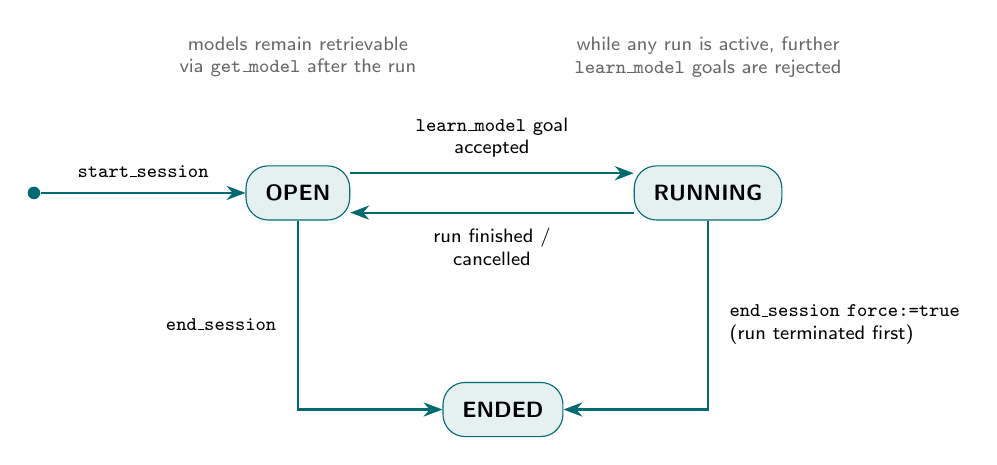
\begin{tikzpicture}

  \node[circle, fill=ros2Accent, inner sep=1.6pt] (init) {};
  \node[ros2/state, right=26mm of init] (open) {OPEN};
  \node[ros2/state, right=36mm of open] (running) {RUNNING};
  \node[ros2/state] (ended) at ($(open.south)!0.5!(running.south) + (0,-24mm)$) {ENDED};

  % ---------------- creation ----------------
  \draw[ros2/accent arrow] (init) -- (open)
    node[ros2/lbl, midway, above=0.7mm]{\texttt{start\_session}};

  % ---------------- OPEN <-> RUNNING ----------------
  \draw[ros2/accent arrow] ([yshift=2.5mm]open.east) -- ([yshift=2.5mm]running.west)
    node[ros2/lbl, midway, above=0.7mm, align=center]
    {\texttt{learn\_model} goal\\accepted};
  \draw[ros2/accent arrow] ([yshift=-2.5mm]running.west) -- ([yshift=-2.5mm]open.east)
    node[ros2/lbl, midway, below=0.7mm, align=center]{run finished /\\cancelled};

  % ---------------- closing ----------------
  % Elbows: straight down, then horizontally into ENDED; labels sit beside
  % the vertical segments.
  \coordinate (lcorner) at (open.south |- ended.west);
  \draw[ros2/accent arrow] (open.south) -- (lcorner) -- (ended.west);
  \node[ros2/lbl, anchor=east, xshift=-1.5mm]
    at ($(open.south)!0.55!(lcorner)$) {\texttt{end\_session}};

  \coordinate (rcorner) at (running.south |- ended.east);
  \draw[ros2/accent arrow] (running.south) -- (rcorner) -- (ended.east);
  \node[ros2/lbl, anchor=west, align=left, xshift=1.5mm]
    at ($(running.south)!0.55!(rcorner)$)
    {\texttt{end\_session} \texttt{force:=true}\\
     {\scriptsize(run terminated first)}};

  % ---------------- annotations ----------------
  \node[ros2/lbl, text=black!60, align=center, above=10mm of open.north]
    {models remain retrievable\\via \texttt{get\_model} after the run};
  \node[ros2/lbl, text=black!60, align=center, above=10mm of running.north]
    {while any run is active, further\\\texttt{learn\_model} goals are rejected};

\end{tikzpicture}

  \caption{Session lifecycle. A session returns to \textsc{open} after a run,
    keeping its results retrievable; closing it is an explicit, separate
    operation.}
  \label{ros2:fig:lifecycle}
\end{figure}

\subsection{Workspace staging and core invocation}
\label{ros2:sec:staging}

The workspace layout reproduces the core's directory conventions:

\begin{lstlisting}[style=ros2iface]
<session workspace>/
  data/         # training + validation CSV (staged copies)
  topologies/   # master topology file
  configs/      # constraints file (only when supplied)
  results/      # results directory targeted by the run
  logs/         # stdout/stderr of the ANSR subprocess
\end{lstlisting}

The core is invoked exactly as in a manual run: bare filenames for the
inputs, the workspace as the working directory, and only the five exposed
parameters on the command line. The subprocess environment pins the
numerical libraries to one thread per worker process
(\texttt{OMP\_NUM\_THREADS=1} and related variables), so the computational
footprint of a run equals its worker pool and remains predictable on a
shared robot computer. Staged copies also make the mid-run data update
self-contained: the update rewrites the staged file atomically under the
same name, which is precisely the event the core's data monitoring watches
for.

\subsection{Process supervision}
\label{ros2:sec:supervision}

A learning run is a small tree of processes: the core's main process, the
Dask scheduler it hosts, and the worker pool, whose members are recycled by
the core over the course of a run as part of its resource management. The
supervisor therefore manages the run at the granularity of its
\emph{process group}, which is invariant across worker recycling: the
subprocess is started as a new session leader, and all lifecycle operations
address the group as a whole.

Termination --- used by action cancellation, forced session closing, and the
wall-time watchdog alike --- follows the two-stage escalation of
Algorithm~\ref{ros2:alg:terminate}: a cooperative \texttt{SIGTERM} to the
whole group, a configurable grace period, then a definitive \texttt{SIGKILL}
for any remainder. The supervisor verifies that no process of the group
survives, so a cancelled run never leaves workers behind. This guarantee is
exercised by a dedicated integration test
(Section~\ref{ros2:sec:verification}).

\begin{algorithm}[tb]
  \caption{Two-stage termination of a learning run's process group.}
  \label{ros2:alg:terminate}
  \KwIn{process group $g$ of the run, grace period $T$}
  send \texttt{SIGTERM} to every process in $g$\;
  $t_{\mathrm{deadline}} \leftarrow \mathrm{now} + T$\;
  \While{$\mathrm{now} < t_{\mathrm{deadline}}$}{
    \lIf{no process of $g$ remains}{\Return}
    wait briefly\;
  }
  send \texttt{SIGKILL} to every process in $g$\;
  wait until no process of $g$ remains\;
\end{algorithm}

On the success path, the supervisor simply polls until the core exits and
tolerates the core's unhurried finalisation: the final export is already
complete on disk before the process ends, so the action result can be
assembled reliably. Exit classification distinguishes a completed run, a
cancelled run, and a failed run; in the failure case, the tail of the
subprocess log is attached to the action result's message for diagnosis. As
a safety net for unattended deployments, the node-side wall-time watchdog
(\texttt{max\_run\_seconds}) terminates a run through the same mechanism and
reports it as cancelled.

\subsection{Retrieving models from the export directory}
\label{ros2:sec:mirror}

Within a session's results directory, the core exports its best-so-far
models per population and dataset version:

\begin{lstlisting}[style=ros2iface]
<results>/seed=1/
  archiveIndividuals/current_best_<v>/          # non-dominated solutions
  mainPopulationIndividuals/current_best_<v>/   # live search population
\end{lstlisting}

Each snapshot directory holds one text report and one MATLAB export per
model, plus an overview file summarising the population. The reader
component selects the \emph{highest} version present --- after a mid-run
data update, a new version appears and earlier versions remain as snapshots
of the previous dataset --- and parses the overview together with the
per-model reports into \texttt{AnalyticModel} messages, preserving the
overview's ordering.

Two timing properties follow from the continuous-export design and are
handled by the reader. First, a snapshot that is being refreshed at the
moment of a query may be momentarily incomplete; reads are therefore retried
briefly and degrade gracefully to an empty result with an explanatory
message rather than failing. Second, the export interval bounds the
staleness of any answer (5\,s by default), and immediately after a data
update the new version's snapshot fills up as models are re-evaluated ---
clients polling right after \texttt{set\_session\_data} should expect the
new version to appear within a few export intervals.

\section{Building and running}
\label{ros2:sec:usage}

The module is built like any ROS\,2 workspace, with one addition: the ANSR
scientific stack (PyTorch, Dask, SymPy) lives in a Python virtual
environment created with system site-packages visible, so that both the ROS
client libraries and the scientific stack are importable from one
interpreter.

\begin{lstlisting}[style=ros2shell, caption={Build recipe (Ubuntu 24.04,
  ROS\,2 Jazzy).}, label={ros2:lst:build}]
sudo apt install ros-jazzy-ros-base python3.12-venv \
                 python3-colcon-common-extensions

# venv on the same interpreter ROS Jazzy uses (Python 3.12); the venv is
# used via absolute paths and never needs to be activated
python3.12 -m venv --system-site-packages ~/venvs/ansr

REPO=$(pwd)    # run from the repository root: absolute path for the steps below
~/venvs/ansr/bin/pip install -r $REPO/source_code/requirements.txt

source /opt/ros/jazzy/setup.bash

mkdir -p ~/ros2_ws/src
ln -sfn $REPO/ros2 ~/ros2_ws/src/physics_amm_ros
cd ~/ros2_ws && colcon build --symlink-install
source install/setup.bash    # repeat in every new terminal
\end{lstlisting}

The \texttt{python\_executable} launch argument (first line of
Listing~\ref{ros2:lst:cli}) points the ANSR subprocess at this virtual
environment's interpreter, so that the subprocess runs with the scientific
stack independently of which interpreter serves the node itself; the node
reports the effective interpreter in its startup log.
Listing~\ref{ros2:lst:cli} walks through a complete session with the
standard \texttt{ros2} command-line tools; the same calls are available
programmatically from any ROS\,2 client library.

\begin{lstlisting}[style=ros2shell, caption={A complete session from the
  command line.}, label={ros2:lst:cli}]
ros2 launch physics_amm physics_amm.launch.py \
     python_executable:=~/venvs/ansr/bin/python

# 1. open a session
ros2 service call /physics_amm/start_session \
     physics_amm_msgs/srv/StartSession

# 2. training a new model: send a learning goal (absolute paths)
ros2 action send_goal /physics_amm/learn_model \
     physics_amm_msgs/action/LearnModel \
     "{session_id: '<uuid>', topology_path: '<abs>/topology.txt',
       train_data_path: '<abs>/train.csv',
       valid_data_path: '<abs>/valid.csv',
       constraints_path: '', outfolder: results}" --feedback

# 3. querying: best-so-far models, any time during or after the run
ros2 service call /physics_amm/get_model \
     physics_amm_msgs/srv/GetModel \
     "{session_id: '<uuid>', population: '', max_models: 3}"

# 4. updating: replace the training data mid-run
ros2 service call /physics_amm/set_session_data \
     physics_amm_msgs/srv/SetSessionData \
     "{session_id: '<uuid>', train_data_path: '<abs>/new_train.csv',
       valid_data_path: ''}"

# 5. cancel when satisfied (Ctrl-C on send_goal, or the action API),
#    then close the session
ros2 service call /physics_amm/end_session \
     physics_amm_msgs/srv/EndSession \
     "{session_id: '<uuid>', force: true}"
\end{lstlisting}

Steps 2--4 are exactly the three operation modes announced in D3.7:
training, querying, and updating are one action goal and two service calls.
Data files are headerless comma-separated CSV with the target variable in
the last column.

\section{Verification}
\label{ros2:sec:verification}

ANSR is an asynchronous evolutionary method: the order in which tuned
candidates return from the worker pool depends on scheduling, so two runs
with identical inputs legitimately produce different (equally valid)
expressions. Verification of the ROS layer therefore does not compare
expressions or loss values against a reference run. Instead, the test suite
asserts the \emph{integration contract} --- that the node invokes and
observes the core exactly as a manual invocation would --- and
\emph{invariants} that must hold for any run. This is where integration
defects would actually appear: in the command line, the workspace layout,
the results path, or process lifecycle management, all of which are
deterministic and precisely testable.

Table~\ref{ros2:tab:tests} shows the six test layers.

The layers that execute the core share a set of bundled smoke fixtures:
60~training and 40~validation samples with inputs drawn uniformly from
$[-2,2]$ and \emph{noise-free} targets $y = x_0^2 + x_1$ (plus an alternative
dataset with $y = x_0^2 + 2x_1$ for the mid-run data update of layer~L5),
paired with a minimal master topology that can represent both targets
exactly. Short runs therefore converge to near-zero validation loss, which
keeps the ``did it learn anything?''\ assertions meaningful within
continuous-integration time budgets --- and any significant residual
implicates the integration, not the data.

\begin{table}[tb]
  \centering
  \caption{Test layers of the ROS bundle.}
  \label{ros2:tab:tests}
  \footnotesize
  \begin{tabular}{@{}clllp{5.1cm}@{}}
    \toprule
    \# & Layer & ROS & Speed & What it proves \\
    \midrule
    L1 & command-line contract & no  & ms         & the node invokes ANSR exactly as a human would \\
    L2 & workspace staging     & no  & ms         & the staged layout matches the core's conventions \\
    L3 & reference smoke       & no  & $\sim$1 min & baseline output structure of a direct run \\
    L4 & ROS smoke             & yes & $\sim$1 min & the action reproduces the L3 structure \\
    L5 & data update mid-run   & yes & $\sim$2 min & dataset version advances; queries answer mid-run \\
    L6 & cancellation          & yes & $\sim$30 s  & termination leaves no process of the run behind \\
    \bottomrule
  \end{tabular}
\end{table}

Layers L1 and L2 are fast, deterministic unit tests that run on every
commit; they pin the exact command line (only the five agreed parameters,
bare filenames) and the workspace layout. Layer L4 compares a run driven
through ROS against the direct-invocation baseline of L3 \emph{structurally}
--- same directory tree, same artifact kinds, finite losses --- never by
values. Layer L5 exercises the mid-run data update end-to-end and verifies
that queries are answered while the action is executing. Layer L6 verifies
the process-group termination guarantee of
Section~\ref{ros2:sec:supervision}: after a cancellation, no process of the
run's group remains within seconds. In addition, the packages carry unit
tests for the ROS-agnostic modules and a launch test that brings the node up
through its launcher, meeting the D5.1 requirement of testing both the
module API and the node; together the suites reach the coverage level of
quality Tier~2.

\section{Operational notes and outlook}
\label{ros2:sec:outlook}

\paragraph{One run at a time.} By default the node executes one learning run
at a time (parameter \texttt{max\_concurrent\_runs}, default~1); goals
arriving while a run is active are rejected immediately with an explanatory
message, and the client retries once the slot is free. Serialising runs keeps the CPU footprint of
the module equal to a single worker pool --- a deliberate choice for shared
robot computers, where the module coexists with perception and control. The
cap is a parameter, so a workstation deployment with ample cores may raise
it, giving each session its own isolated workspace and results directory.

\paragraph{Termination policy.} Learning is an anytime computation: the
best-so-far models are continuously available, so clients decide when the
result is good enough and cancel. The node-side watchdog
(\texttt{max\_run\_seconds}) bounds unattended runs; its default equals the
core's own time budget, so it acts purely as a safety net.

\paragraph{Outlook.} Three integration steps are foreseen. First, the
\texttt{AnalyticModel} message was designed field-compatible with
\texttt{ModelDescription} in \texttt{coresense\_msgs}, so migrating to the
shared CoreSense types once the consortium consolidates interfaces is a
mechanical mapping. Second, the module ships its own launcher and default
configuration, ready to be composed into a system-level bringup
(\texttt{coresense\_bringup}). Third, following the D5.1 release process,
the packages will be released with \texttt{bloom} from the
\texttt{jazzy-devel} branch once the interface has settled in consortium
use.


\bibliographystyle{unsrt}
\bibliography{ros2-chapter/refs}

\end{document}
